%\chapter{Spherical Harmonics}
\chapter{球谐函数}
\label{chapter:sh}

球谐函数是单位球面上正交归一的基函数。
由于地球接近球形,因此,这些函数在地球物理学的许多分支中扮演重要角色是毫不奇怪的。 大规模数据如外部重力势和基本地磁场的规约处理,
以及如地球内部三维压缩或剪切波速度或核幔边界以下熔融的富铁物质的流速的模型或理论预测,这些结果通常都是用球谐函数展开的。
此外,球谐函数自然地出现在球对称无自转地球模型的弹性-重力自由振荡的分析中;
它们使运动方程分离成环型和球型的两组普通径向标量方程,可以进行数值积分。

贯穿全书,我们始终强调实数球谐函数~$\sY_{lm}$~的使用,
\index{spherical harmonics!real}%
\index{real spherical harmonics}%
因为它们是在模式分裂和耦合计算中最自然也最方便的基。但是,我们在本附录中首先
定义{\em 复数\/}球谐函数~$Y_{lm}$。
\index{spherical harmonics!complex}%
\index{complex spherical harmonics}%
我们用来构建和分析这些函数的操作方法是基于角动量的量子力学理论。
Edmonds (\citeyear{edmonds60})~的简洁的经典专着
为这一题目提供了极好的易于上手的入门读物;
Varshalovich, Moskalev \& Khersonskii (\citeyear{varshalovich&al88})~ 有更为详尽的讨论。在本附录中我们对球谐函数的概述与最近另一部也是针对地球物理学家的专著(Backus, Parker \& Constable {\citeyear{backus&al96})~相似。
他们的处理比我们的更具教学的氛围,因为在他们讨厌"可以证明"这种语言。
然而,我们讨论了一些他们所遗漏的但与全球地震学有关的议题,包括实数矢量球谐函数~$\bP_{lm},\bB_{lm},\bC_{lm}$ \vspace{-0.2 ex}
以及复数次数的行波球谐函数~$Q_{\lambda m}^{(1)}$、$Q_{\lambda m}^{(2)}$。

最后再引入一个有用的符号元素:一个单位球~$\Omega$~上的复数标量函数~$\psi$~如果满足
\eq \label{B.squint}
\int_{\Omega}\psi^*\psi\,d\/\Omega<\infty,
\en
则~$\psi$~被称为是{\em 平方可积\/}的,
\index{square integrability}%
式中星号表示复共轭。两个平方可积函数~$\psi$~和~$\chi$~的{\em 内积\/}的定义为
\index{inner product!of scalar fields}%
\eq
\label{B.inprod}
\langle\psi,\chi\rangle=\int_\Omega \psi^*\chi\,d\Om.
\en
如果~$\langle\psi,\chi\rangle=0$,则称~$\psi$~和~$\chi$~这两个函数为{\em 正交的\/}。
\index{orthogonality!of scalar fields}%
单一函数~$\psi$~的{\em 范数\/}~$\|\psi\|$~
\index{norm!on the unit sphere}%
为~$\|\psi\|=\langle\psi, \psi\rangle^{1/2}$。
如果函数~$\psi$~和~$\chi$~为实数的,(\ref{B.squint})~和~(\ref{B.inprod}})~式中的星号
可以省略。在第~A.7~节中归纳了这里所采用的单位球的几何性质。

%\section{Harmonic Homogeneous Polynomials}
\section{调和齐次多项式}
\index{homogeneous polynomial!harmonic|(}%
\label{section:harpol}

次数为~$l$~的{\em 齐次多项式\/}
\index{homogeneous polynomial}%
是三维空间中的位置~$\br=x\bxh+y\byh+z\bzh$~的实数或复数函数,其形式为
\eq \label{B.harmpol}
H_l(\br)=\sum_{\alpha,\beta,\gamma}C_{\alpha\beta\gamma}x^\alpha
y^\beta z^\gamma,
\en
其中~$\alpha$、$\beta$~和~$\gamma$~为非负整数,它们须满足
\eq \label{B.totdegl}
\alpha+\beta+\gamma=l.
\en
(\ref{B.totdegl})~这一条件限定了求和式~(\ref{B.harmpol})中的每个单项式的总次数都是~$l$;故称为"齐次"。一个复数多项式有\textcolor{red}{实数}系数~$C_{\alpha\beta\gamma}$,
而实数多项式则有\textcolor{red}{复数}系数~$C_{\alpha\beta\gamma}$。
每个齐次多项式在半径为~$r$~的球面上的值,可以从它在单位球面~$\Omega$~ 上的值通过以下关系来决定:
\eq H_l(\br)=r^l\sum_{\alpha,\beta,\gamma}
C_{\alpha\beta\gamma}\left(\frac{x}{r}\right)^\alpha
\left(\frac{y}{r}\right)^\beta
\left(\frac{z}{r}\right)^\gamma=r^lH_l(\brh).
\en
次数为~$l$~的实数或复数齐次多项式空间的维度是 $\half(l+1)(l+2)$,因为这就是满足约束条件~(\ref{B.totdegl})~的独立非
负整数~$\alpha$、$\beta$、$\gamma$~组合的数目。

一个~$l$~次的{\em 调和齐次多项式\/}
\index{harmonic homogeneous polynomial}%
\index{homogeneous polynomial!harmonic}%
是一个满足拉普拉斯方程:
\eq
\del^2Y_l=0. \label{eq:defsolsph}
\en
的~$l$~次齐次多项式~$Y_l(\br)$。
\index{degree}%
\index{spherical harmonics!degree of}%
遵循~\textcite{kellogg67},我们可以通过考虑以下表达式
\eq \label{B.Kellogg}
Y_l=a_l+a_{l-1}z+\cdots+a_0z^l,
\en
来确定调和齐次多项式空间的维度,这里每个~$a_s$~都是~$x$~和~$y$~的~$s$~次齐次多项式。
从使~(\ref{B.Kellogg})~式为调和的条件~(\ref{eq:defsolsph})~
可以得到多项式~$a_s$~满足的一系列递推关系。因此我们有
\eqa \label{B.Kellogg2}
\lefteqn{Y_l=a_l+a_{l-1}z-\frac{1}{2!}z^2\del^2a_l
-\frac{1}{3!}z^3\del^2a_{l-1}} \nonumber \\
&&\mbox{}\qquad\qquad+\frac{1}{4!}z^4\del^2\del^2a_l
+\frac{1}{5!}z^5\del^2\del^2a_{l-1}-\cdots.
\ena
从~(\ref{B.Kellogg2})~我们可以发现~$Y_l$~完全由最前面的两个多项式~$a_l(x,y)$和~ $a_{l-1}(x,y)$~所决定。对于~$a_l$~和~$a_{l-1}$~分别有~$l+1$~个和~$l$~ 个线性独立的选择;因此实数或复数调和齐次多项式空间的维度是~$2l+1$。$l$~次 调和齐次多项式~$Y_l$~的另一个名称是{\em 立体球谐函数\/}。
\index{solid spherical harmonic}%
\index{spherical harmonics!solid}%

用归纳法可以证明每一个~$l$~次齐次多项式都可以用如下形式写为立体球谐函数~ 
$Y_l,Y_{l-2},\ldots$~的唯一的线性组合
\eq
H_l=\left\{\begin{array}{ll}
Y_l+r^2Y_{l-2}+\cdots+r^lY_0 & \mbox{若 $l$ 为偶数} \\
\vspace{-0.8 ex} & \vspace{-0.8 ex} \\
Y_l+r^2Y_{l-2}+\cdots+r^{l-1}Y_1 & \mbox{若 $l$ 为奇数.}
\end{array}\right.
\en
合并同类项,我们也可以将~$H_l$~用一个唯一的~$l$~次立体球谐函数和 一个唯一的~$l-2$~次非调和齐次多项式来表示:
\eq \label{B.HeqY}
H_l=Y_l+r^2H_{l-2}.
\en
包含直接求和分解式~(\ref{B.HeqY})~中函数~$H_l$~和~$r^2H_{l-2}$~的空间的维度分别为~ $\half(l+1)(l+2)$~和~$\half (l-1)l$;
这也为立体或表面球谐函数~$Y_l$~的维度是~$2l+1$~提供了另一个证明。

利用关系~$Y_l(\br)=r^lY_l(\brh)
=r^lY_l(\theta,\phi)$,将立体球谐函数限定在单位球面上的点~ $\brh=(\theta,\phi)$,得到的结果被称为{\em 表面球谐函数\/}。
\index{surface spherical harmonics}%
\index{spherical harmonics!surface}%
我们以相同的符号来表示立体和表面球谐函数,仅用自变量来区分函数~$Y_l(\br)$~与~ $Y_l(\brh)=Y_l(\theta,\phi)$,或者当没有给出自变量时由上下
文决定。将拉普拉斯方程~(\ref{eq:defsolsph})~展开为 $[\p_r^2+2r^{-1}\p_r+r^{-2}\del_1^2]
[r^lY_l(\theta,\phi)]=0$,我们发现所有~$l$~次表面球谐函数均满足{\em 球坐标亥姆霍兹方程\/}
\index{spherical Helmholtz equation}%
\index{Helmholtz equation!spherical}%
\eqa \label{B.delsqY} \lefteqn{
\del_1^2Y_l+l(l+1)Y_l} \nonumber \\
&&\mbox{}=[\p_{\theta}^2+\cot\theta\,\p_{\theta}
+(\sin\theta)^{-2}\p_{\phi}^2+l(l+1)]Y_l=0.
\ena
只要愿意,我们也可以通过寻求偏微分方程~(\ref{B.delsqY})~的分离变量解
来构建一组由~$2l+1$~个线性独立的~$l$~次表面球谐函数所组成的基。
然而在此我们介绍一个利用量子力学中角动量算子特性的{\em 纯代数的\/}建构程序。在附录~C~中,
我们将展示如何通过考虑自旋以及轨道角动量将这种代数方法推广到
矢量和更高阶的张量球谐函数。
\index{homogeneous polynomial!harmonic|)}%

%\section{Angular-Momentum Operator}
\section{角动量算子}
\index{angular momentum|(}%
\label{section:angmom}

量子力学中的可观测量是以厄米特线性算子表示的;动量算子为~ $-i\hbar\bdel$,与其对应的角动量算子为~ $-i\hbar(\br\times\bdel)=-i\hbar(\brh\times\bdel_1)$。
后一个算子是复数表面球谐函数分析的基本要素;
由于我们对量子力学应用不感兴趣,我们设普朗克常数~$\hbar$~为~1,并将无量纲矢量
\eq \label{B.Ldef}
\bL=-i(\brh\times\bdel_1)=
i[\bthetah(\sin\theta)^{-1}\p_{\phi}-\bphih\p_{\theta}]
\en
称为{\em 角动量算子\/}。
\index{angular-momentum operator}%
\index{operator!angular-momentum}%

我们可以将~$\bL$~视为一个作用在~$r,\theta,\phi$~的标量函数上的三维
算子,或是一个局限于单位球面~$\Omega$~上的二维算子;在后一种场合,
它将仅依赖于~$\theta,\phi$~的标量场映射到切向矢量场:$\brh\cdot\bL=0$。
角动量算子的平方~$L^2=\bL\cdot\bL$~是负的表面拉普拉斯算子:
\index{surface Laplacian}%
\index{Laplacian!surface}%
\eq \label{B.Lsq2}
L^2=-\del_1^2=-[\p_{\theta}^2+\cot\theta\,\p_{\theta}
+(\sin\theta)^{-2}\p_{\phi}^2].
\en
在笛卡尔坐标~$x,y,z$~中,我们可以把算子~$\bL$~和~$L^2$~写为
\eq \label{B.Ldef3}
\bL=\bxh L_x+\byh L_y+\bzh L_z,\qquad L^2=L_x^2+L_y^2+L_z^2,
\en
其中
\eqa \label{B.LxLyLz}
\lefteqn{L_x=-i(y\p_z-z\p_y),
\qquad L_y=-i(z\p_x-x\p_z),} \nonumber \\
&&\mbox{}\qquad\qquad
L_z=-i(x\p_y-y\p_x).
\ena
使用球极坐标表达式~(\ref{B.Ldef})~或笛卡尔坐标表达式~(\ref{B.Ldef3})~可以很容易证明
\eq \label{A.LxLiL}
\bL\times\bL=i\bL.
\en

两个任意标量或矢量线性算子~$\sA$~和~$\sB$~的{\em 对易子\/}的定义为
\index{commutator}%
\eq \label{B.commdef}
[\sA,\sB]=\sA\hspace{0.2 mm}\sB-\sB\sA.
\en
显然,$[\sA,\sB]=-[\sB,\sA]$。如果~$[\sA,\sB]$~为零,我们说算子~$\sA$~和~$\sB$~ 
为{\em 可易的\/}。可易性的概念在量子力学中扮演了根本的角色:当且仅当两个可观测量的算子为可易时,它们具有共同的本征函数基,且可以被同时确定而不会违背海森堡测不准原理。
角动量的叉乘积关系~(\ref{A.LxLiL})~可以用对易子符号~(\ref{B.commdef})~ 写成以下形式
\eq \label{B.comm2}
[L_x,L_y]=iL_z,\qquad[L_y,L_z]=iL_x,\qquad[L_z,L_x]=iL_y.
\en
(\ref{B.comm2})~显示笛卡尔分量~$L_x$、$L_y$、$L_z$~互相之间是不可易的。
另一方面,可以很容易验证~$L^2$~与~$\bL$~是可易的,因而与任一分量也是可易的:
\eq
[L^2,L_x]=[L^2,L_y]=[L^2,L_z]=0.
\label{eq:l2l}
\en
因此,角动量~$\bL$~的两个正交分量不能同时被确定;但是,它的平方~$L^2$~及其任
何一个分量是可以的。从定义~(\ref{B.Ldef})~中可以明确看出,$\bL$~与~ $\p_r$~以及任何仅依赖于半径的标量或矢量函数~$f(r)$~是可易的:
$[\p_r,\bL]=\bzero$及$[f(r),\bL]=\bzero$.
从这一结果以及球极坐标形式的拉普拉斯算子~ $\del^2=\p_r^2+2r^{-1}\p_r+r^{-2}\del_1^2$,我们~有$[\del^2,\bL]=\bzero$。
(\ref{eq:l2l})~表明,表面拉普拉斯算子和表面旋度算子是可易的: $[\del_1^2,\brh\times\bdel_1]=\bzero$。另一方面,表面
拉普拉斯算子和表面梯度算子之间不可易;事实上,有~$[\del_1^2,\bdel_1]=-2\brh\,\del_1^2$。

在下一节中,我们将借助于两个{\em 阶梯算子\/}
\index{ladder operator}%
\index{operator!ladder}%
\eq \label{B.ladder}
L_+=L_x+iL_y,\qquad L_-=L_x-iL_y,
\en
来构建单位球上的一组正交归一基函数。
算子~$L_\pm$~满足的对易关系为
\index{angular-momentum operator!commutation relations}%
\index{commutation relations}%
\eq \label{eq:commu1}
[L^2,L_\pm]=0,\qquad
[L_z,L_{\pm}]=\pm L_{\pm},\qquad
[L_+,L_-]=2L_z.
\en
我们可以用~$L_\pm$~和~$L_z$~将~$L^2$~表示为下面两种形式的任何一个
\eq
L^2=L_+L_-+L_z^2-L_z=L_-L_++L_z^2+L_z. \label{eq:L2}
\en
利用~(\ref{B.Ldef})~和几何关系~(\ref{A.need1})--(\ref{A.need2}),可以得到球极坐标中~$L_x$、$L_y$~和~$L_z$~的显式表达式:
\eq
L_x=i(\sin\phi\,\p_\theta+\cot\theta\cos\phi\,\p_\phi),
\label{eq:Lxtp}
\en
\eq
L_y=i(-\cos\phi\,\p_\theta+\cot\theta\sin\phi\,\p_\phi),
\label{eq:Lytp}
\en
\eq
L_z=-i\p_\phi. \label{eq:Lztp}
\en
阶梯算子~(\ref{B.ladder})~的相应表达式为
\eq \label{B.sphlad}
L_\pm=e^{\pm i\phi}(\pm\p_\theta+i\cot\theta\,\p_\phi).
\en
取~(\ref{B.sphlad})~的复共轭,我们看到~$(L_{\pm})^*=-L_{\mp}$。

如果~$\sA$~为一个将单位球~$\Omega$~映射到其自身的标量或矢量算子,它的{\em 伴随\/}算子~$\sA^{\dagger}$~的定义为
\index{adjoint operator}%
\index{operator!adjoint}%
$\langle\psi,\sA\chi\rangle=\langle\sA^{\dagger}\psi,\chi\rangle$。
显而易见,取该关系的复共轭可得~$(\sA^{\dagger})^{\dagger}=\sA$。
角动量算子~(\ref{B.Ldef})~是一个{\em 自伴随}或{\em 厄米特\/}算子:
\index{self-adjoint operator}%
\index{Hermitian operator}%
\index{operator!self-adjoint}%
\index{operator!Hermitian}%
\eq \label{B.LHerm}
\bL^\dagger=\bL.
\en
对~(\ref{B.LHerm})~的证明最直接的是其~$L_z$~分量:
\eqa \label{B.Hermproof}
\lefteqn{\langle\psi,L_z\chi\rangle=
\int_\Omega\psi^*(L_z\chi)\,d\Om=
\int_\Omega\psi^*(-i\p_{\phi}\chi)\,d\Om} \nonumber \\
&&\mbox{}=\int_\Omega(-i\p_{\phi}\psi)^*\chi\,d\Om
=\int_\Omega(L_z\psi)^*\chi\,d\Om=\langle L_z\psi,\chi\rangle.
\ena
这里我们对经度~$\phi$~进行了分部积分来得到第三个等式。由于坐标轴~$\bxh$、$\byh$、 $\bzh$~可以任意选取,算子~$L_x$~和~$L_y$~也均为厄米特算子; 这一点可以利用表达式~(\ref{eq:Lxtp})--(\ref{eq:Lytp})~并对~$\theta$~和~ $\phi$~进行分部积分而直接验证。同样可以证明角动量平方算子也是厄米特算子: $(L^2)^\dagger=(\bL\cdot\bL)^\dagger=\bL^\dagger\cdot\bL^\dagger
=\bL\cdot\bL=L^2$。而两个阶梯算子互为彼此的伴随算子:$(L_{\pm})^\dagger=L_{\mp}$。
\index{angular momentum|)}%

%\section{Construction of a Basis}
\section{基的构建}
\index{spherical harmonics!basis construction|(}%
\label{sec:conbas}

厄米特算子的本征值均为实数,且相应的本征函数相互正交。
因此,我们就利用厄米特算子~$L^2$~和~$L_z$~来构建复数表面球谐函数的基。
可易性~$[L^2,L_z]=0$~确保我们能够找到这两个算子的共同本征函数。
我们用第二个称为{\em 级数\/}的角标~$m$~来区分这这些本征函数,写为
\index{order}%
\index{spherical harmonics!order of}%
\eq \label{B.simult}
L^2Y_{lm}=l(l+1)Y_{lm},\qquad L_zY_{lm}=mY_{lm}.
\en
将~$L_z$~的球极坐标表达式~(\ref{eq:Lztp})~代入~(\ref{B.simult})~中第二个本征值方程,我们发现每个基都必须有如下形式
\eq \label{B.Xlmdef}
Y_{lm}(\theta,\phi)=X_{lm}(\theta)\exp(im\phi).
\en
从~(\ref{B.Xlmdef})~可以看到,为保证~$Y_{lm}$~的单值性,级数~$m$~必须为整数。

利用对易关系~(\ref{eq:commu1}),很容易证明函数~$L_\pm Y_{lm}$~是~$L^2$~和~$L_z$~的
共同本征函数,且相应的本征值分别为~$l(l+1)$~和~$m\pm 1$:
\eq \label{B.LADDER}
L^2(L_\pm Y_{lm})=L_\pm(L^2 Y_{lm})=l(l+1)(L_\pm Y_{lm}),
\en
\eq
L_z(L_\pm Y_{lm})=(L_\pm L_z\pm L_\pm) Y_{lm}
=(m\pm 1)(L_\pm Y_{lm}).
\label{eq:Lladder}
\en
现在我们可以看到如此命名的原因:{\em 升阶\/}算子~$L_+$~ 
\index{ladder operator!ascending}%
\index{operator!ladder!ascending}%
将~$Y_{lm}$~变换为常数乘以~$Y_{l\,m+1}$,
而{\em d降阶\/}算子~$L_-$~将~$Y_{lm}$~变换为常数乘以~$Y_{l\,m-1}$:
\index{ladder operator!descending}%
\index{operator!ladder!descending}%
\eq \label{B.LpmYlm}
L_\pm Y_{lm}=c_{\pm}Y_{l\,m\pm1}.
\en
变换后函数~$L_\pm Y_{lm}$~的平方范数与~$Y_{lm}$~的平方范数有关系:
\eqa \lefteqn{\|L_\pm Y_{lm}\|^2=
\langle L_{\pm}Y_{lm}, L_{\pm}Y_{lm}\rangle
=\langle Y_{lm},L_{\mp}L_{\pm}Y_{lm}\rangle} \nonumber \\
&&\mbox{}=\langle Y_{lm},(L^2-L_z^2\mp L_z)Y_{lm}\rangle \nonumber \\
&&\mbox{}\qquad=(l\mp m)(l\pm m+1)\,\| Y_{lm}\|^2. \label{B.Ylmpm}
\ena
由于只有当一个函数恒为零时该函数的范数才会为零,因此有~$L_{\pm}Y_{l\,\pm l}=0$。
无论是升阶还是降阶,持续下去都有一个自然的终点;
$L_z$~的本征值局限在~$-l\leq m\leq l$~的范围内。
因此,每一个整数次数~$0\leq l\leq\infty$~有~$2l+1$~个表面球谐函数基~$Y_{lm}$。

$L^2$~和~$L_z$~的厄米特性质确保不同次数~$l\neq l'$~和不同级数~$m\neq m'$~的球谐函数~$Y_{lm}$和$Y_{l'm'}$~ 
是正交的。我们进一步规定,每个基必须为单位长度;这使得所有基都是{\em 正交归一\/}的:
\index{orthonormal basis}%
\index{basis!orthonormal}%
\index{spherical harmonics!orthonormality}%
\eq
\langle Y_{lm},Y_{l'm'}\rangle=\int_\Omega
Y_{lm}^*Y^{}_{l'm'}\,d\Om=\delta_{ll'}\delta_{mm'}.
\label{eq:ortho}
\en
在~(\ref{B.Ylmpm})~中当~$-l\leq m\leq l$~时 令~$\|Y_{lm}\|^2=1$,并利用~(\ref{B.LpmYlm}),
我们得到~$|c_{\pm}|^2=(l\mp m)(l\pm m+1)$。
平方根~$c_{\pm}$~的符号可以任意选择。

从~$L_{\pm}Y_{l\,\pm l}=
e^{\pm i\phi}(\pm\p_\theta+i\cot\theta\,\p_\phi)
[X_{l\,\pm l}(\theta)e^{\pm il\phi}]=0$~这个条件我们得到一个常微分方程
\eq \label{B.Xlleqn}
\left (\frac{d}{d\/\theta}-l\cot\theta\right )\!X_{l\,\pm l}=0.
\en
它可以用来确定级数最高和最低的本征函数对余纬度的依赖性。
方程~(\ref{B.Xlleqn})~的解为~$X_{l\,\pm l}=A_{\pm}(\sin\theta)^l$。积分常数~ $A_{\pm l}$~可以用归一化条件~$\|Y_{l\,\pm l}\|^2=1$~确定,符号仍然是不确定的。
以最低级本征函数~$Y_{l\,-l}$~作为第一个正交归一基,并用升阶算子來构建其余的基~ $Y_{l\,-l-1},\ldots, Y_{l0},\ldots,Y_{ll}$,我们定义
\eq \label{eq:first}
Y_{l-l}=\left(\frac{2l+1}{4\pi}\right)^{\!1/2}\frac{\sqrt{(2l)!}}
{2^ll!}(\sin\theta)^l\,e^{-il\phi}
\en
和
\eq \label{eq:def1}
Y_{lm}=\left[\frac{(l-m)!}{(l+m)!}\right]^{1/2}
\left[\frac{1}{(2l)!}\right]^{1/2}(L_+)^{l+m}\,Y_{l\,-l},
\en
这里我们选择了符号~${\rm sgn}\,A_-=1$~和~${\rm sgn}\,c_+=1$。
我们也可以将最高级本征函数~$Y_{ll}$~
作为第一个基,并用降阶算子来构建其余的基~$Y_{l\,l-1},\ldots,
Y_{l0},\ldots,Y_{l\,-l}$;再选择符号为~${\rm sgn}\,A_+=(-1)^l$~和~${\rm sgn}\,c_-=1$~便得到另一种等价于~(\ref{eq:first})--(\ref{eq:def1})~的定义:
\eq \label{eq:last}
Y_{ll}=(-1)^l\left(\frac{2l+1}{4\pi}\right)^{\!1/2}
\frac{\sqrt{(2l)!}}{2^ll!}(\sin\theta)^l\,e^{il\phi}
\en
和
\eq \label{eq:def2}
Y_{lm}=\left[\frac{(l+m)!}{(l-m)!}\right]^{1/2}
\left[\frac{1}{(2l)!}\right]^{1/2}(L_-)^{l-m}\,Y_{ll},
\en
由此得到的基函数满足本征值方程~(\ref{B.simult})~和正交归一化条件~(\ref{eq:ortho})~以及阶梯关系
\eq \label{B.ladfin}
L_{\pm}Y_{lm}=\sqrt{(l\mp m)(l\pm m+1)}\,Y_{l\,m\pm 1}.
\en
通过定义当~$|m|>l$~时~$Y_{lm}=0$,(\ref{B.ladfin})~式将对所有的~$m$~都成立。
这里我们所做的符号选择来自\textcite{condon&shortley35}
和~\textcite{edmonds60}。

\begin{table}[!b]
\centering
\begin{tabular}{|ll|c|c|} \hline
&&& \\
$l$ &  \hspace{-3.0 mm} $m$  &     $Y_{lm}(\brh)$  &   $Y_{lm}(\br)$ \\
&&& \\ \hline
     &        &                     & \\
$0$ &   \hspace{-2.0 mm} $0$  &  $\frac{1}{2\sqrt{\pi}}$  &
$\frac{1}{2\sqrt{\pi}}$  \\
&&& \\
$1$ &  \hspace{-2.0 mm} $0$  &  $\half\sqrt{\frac{3}{\pi}}\cos\theta$  &
  $\half\sqrt{\frac{3}{\pi}}\,z$ \\
&&& \\
$1$ &    \hspace{-4.5 mm} $\pm 1$  &
$\mp\half\sqrt{\frac{3}{2\pi}}\sin\theta\,e^{\pm i\phi}$
 &  $\mp\half\sqrt{\frac{3}{2\pi}}\,(x\pm iy)$ \\
&&& \\
$2$  &    \hspace{-2.0 mm} $0$  &
$\quart\sqrt{\frac{5}{\pi}}\,(3\cos^{2\!}\theta-1)$
  &  $\quart\sqrt{\frac{5}{\pi}}\,(2z^2\hspace{-0.3 mm}
-x^2\hspace{-0.3 mm}-y^2)$ \\
&&& \\
$2$  &     \hspace{-4.5 mm} $\pm 1$  & $\mp\half\sqrt{\frac{15}{2\pi}}
  \sin\theta\cos\theta\,e^{\pm i\phi}$  &
  $\mp\half\sqrt{\frac{15}{2\pi}}\,z(x\pm iy)$ \\
&&& \\
$2$  &     \hspace{-4.5 mm} $\pm 2$  & $\quart\sqrt{\frac{15}{2\pi}}
   \sin^{2\!}\theta\,e^{\pm 2i\phi}$
  &  $\quart\sqrt{\frac{15}{2\pi}}\,(x\pm iy)^2$ \\
&&& \\
$3$  &     \hspace{-2.0 mm} $0$  & $\quart\sqrt{\frac{7}{\pi}}
   \cos\theta\,(5\cos^{2\!}\theta-3)$
  &  $\quart\sqrt{\frac{7}{\pi}}\,z(2z^2\hspace{-0.3 mm}
-3x^2\hspace{-0.3 mm}-3y^2)$ \\
&&& \\
$3$  &     \hspace{-4.5 mm} $\pm 1$  & $\mp\eighth\sqrt{\frac{21}{\pi}}
    \sin\theta\,(5\cos^{2\!}\theta-1)\hspace{0.3 mm}e^{\pm i\phi}$
  &  $\mp\eighth\sqrt{\frac{21}{\pi}}\,(x\pm iy)
(4z^2\hspace{-0.3 mm}-x^2\hspace{-0.3 mm}-y^2)$ \\
&&& \\
$3$  &    \hspace{-4.5 mm}  $\pm 2$  & $\quart\sqrt{\frac{105}{2\pi}}
   \cos\theta\sin^{2\!}\theta\,e^{\pm 2i\phi}$
  &  $\quart\sqrt{\frac{105}{2\pi}}\,z(x\pm iy)^2$ \\
&&& \\
$3$  &     \hspace{-4.5 mm} $\pm 3$  & $\mp\eighth\sqrt{\frac{35}{\pi}}
   \sin^{3\!}\theta\,e^{\pm 3i\phi}$
  &  $\mp\eighth\sqrt{\frac{35}{\pi}}\,(x\pm iy)^3$ \\
     &        &                     & \\ \hline
\end{tabular}
\caption[table:spherharms]
{次数~$l$~为~0~到~3~的复数表面球谐函数~$Y_{lm}(\hat{\bf r})$~及相应的立体球谐函数~$Y_{lm}({\bf r})=r^lY_{lm}(\hat{\bf r})$。}
\label{table:sph}
\end{table}
要得到表面球谐函数~$Y_{lm}$~的显式表达式,我们需要确定算子~$L_-$~和~$L_+$~ 
分别重复作用于~$Y_{ll}$~和~$Y_{l\,-l}$~的结果。用归纳法很容易证明
\eqa \label{B.Jpmugly} \lefteqn{
(L_{\pm})^{l\pm m}\left[(\sin\theta)^le^{\mp il\phi}\right]=
(\sin\theta)^{\pm m}} \nonumber \\
&&\mbox{}\qquad\times\left(\pm\frac{1}{\sin\theta}
\frac{d}{d\theta}\right)^{l\pm m}(\sin\theta)^{2l}e^{im\phi}.
\ena
因此,(\ref{eq:first})--(\ref{eq:def1})~和~(\ref{eq:last})--(\ref{eq:def2})~等价于
\eqa \label{B.Ylm2defs}
\lefteqn{Y_{lm}=\left(\frac{2l+1}{4\pi}\right)^{\!1/2}\frac{1}{2^ll!}
\left[\frac{(l-m)!}{(l+m)!}\right]^{1/2}} \nonumber \\
&&\qquad\mbox{}\times (\sin\theta)^{m}
\left(\frac{1}{\sin\theta}\frac{d}{d\theta}\right)^{l+m}
(\sin\theta)^{2l}e^{im\phi} \nonumber \\
&&\!\!\mbox{}=(-1)^l\left(\frac{2l+1}{4\pi}\right)^{\!1/2}\frac{1}{2^ll!}
\left[\frac{(l+m)!}{(l-m)!}\right]^{1/2} \nonumber \\
&&\qquad\mbox{}\times (\sin\theta)^{-m}
\left(-\frac{1}{\sin\theta}\frac{d}{d\theta}\right)^{l-m}
(\sin\theta)^{2l}e^{im\phi}.
\ena
比较上述两个表达式,我们得到一个重要关系
\eq \label{B.Ylmstar}
Y_{l\,-m}=(-1)^mY_{lm}^*.
\en
由于相应的立体球谐函数~$Y_{lm}(\br)=r^lY_{lm}(\brh)$~为~ $l$~次齐次多项式,我们还必须有~$Y_{lm}(-\brh)=(-1)^lY_{lm}(\brh)$,
或等价于
\eq
\label{B.Yparity}
Y_{lm}(\pi-\theta,\phi+\pi)=(-1)^lY_{lm}(\theta,\phi).
\en
(\ref{B.Yparity})~这一结果表明,每个 $Y_{lm}$~在倒转变换(穿过原点的反射)下是对称或反对称的,取决于 次数~$l$~是偶数还是奇数。
用量子力学的术语,我们说~$Y_{lm}$~的{\em 宇称\/}是~$(-1)^l$。
\index{parity}%
\index{spherical harmonics!parity of}%
表~B.1~中列出了前几个表面和立体球谐函数的显式公式。
\index{spherical harmonics!basis construction|)}%

%\section{Associated Legendre Functions}
\section{连带勒让德函数}
\index{associated Legendre function|(}%
\index{Legendre function!associated|(}%
\label{B.sec.assLeg}

将表达式$Y_{lm}(\theta,\phi)=
X_{lm}(\theta)e^{im\phi}$代入球面亥姆霍兹方程 $\del_1^2Y_{lm}+l(l+1)Y_{lm}=0$,我们发现
余纬度函数$X_{lm}(\theta)$满足常微分方程
\eq
\frac{d^2\!X}{d\theta^2}+\cot\theta\,\frac{dX}{d\theta}
+\left[l(l+1)-\frac{m^2}{\sin^2\theta}\right]\!X=0.
\label{eq:Legeqn}
\en
\index{Legendre's equation}%
变量替换$\mu=\cos\theta$将其转变为{\em 勒让德方程\/}
\eq
(1-\mu^2)\frac{d^2\!X}{d\mu^2}
-2\mu\frac{dX}{d\mu}
+\left[l(l+1)-\frac{m^2}{1-\mu^2}\right]\!
X=0.
\label{eq:Legeqn2}
\en
方程~(\ref{eq:Legeqn2})在$-1\leq\mu\leq 1$区间上的规范解是
次数为$l$、级数为$-l\leq m\leq l$的{\em 连带勒让德函数\/},其定义为
\eq \label{B.Plmdef}
P_{lm}(\mu)=\frac{1}{2^ll!}\,(1-\mu^2)^{m/2}
\left(\frac{d}{d\mu}\right)^{l+m}(\mu^2-1)^l.
\en
这些函数满足固定级数的正交归一化关系
\index{associated Legendre function!orthonormality}%
\eq \label{B.Portho}
\int_{-1}^1P_{lm}(\mu)P_{l'm}(\mu)\,d\mu=
\frac{2}{2l+1}\frac{(l+m)!}{(l-m)!}\,\delta_{ll'}
\en
以及一系列三项递推关系,例如
\index{associated Legendre function!recursion relations}%
\eq
(l-m+1)P_{l+1\,m}-(2l+1)\mu P_{lm}+(l+m)P_{l-1\,m}=0,
\label{eq:stable}
\en
\vspace{-1.0 mm}
\eqa \label{B.Libb1}
\lefteqn{(1-\mu^2)^{1/2}P_{l\,m+1}-2m\mu P_{lm}} \nonumber \\
&&\qquad\mbox{}+(l+m)(l-m+1)(1-\mu^2)^{1/2}P_{l\,m-1}=0,
\ena
\eq \label{B.Libb2}
P_{l+1\,m}-\mu P_{lm}-(l+m)(1-\mu^2)^{1/2}P_{l\,m-1}=0,
\en
\eq
\mu P_{lm}-P_{l-1\,m}-(l-m+1)(1-\mu^2)^{1/2}P_{l\,m-1}=0,
\en
\vspace{-2.5 mm}
\eqa \lefteqn{
(l-m+1)P_{l+1\,m}+(1-\mu^2)^{1/2}P_{l\,m+1}} \nonumber \\
&&\qquad\mbox{}-(l+m+1)\mu P_{lm}=0,
\ena
\[
(l-m)\mu P_{lm}-(l+m)P_{l-1\,m}+(1-\mu^2)^{1/2}P_{l\,m+1}=0.
\]
$P_{lm}$的导数由以下任一等价公式给出
\begin{displaymath}
(1-\mu^2)\frac{dP_{lm}}{d\mu}
=(1-\mu^2)^{1/2}P_{l\,m+1}-m\mu P_{lm}
\end{displaymath}
\vspace{-5.0 mm}
\begin{displaymath}
\qquad\qquad\qquad\hspace{-0.1 mm}\mbox{}
=m\mu P_{lm}-(l+m)(l-m+1)(1-\mu^2)^{1/2}
P_{l\,m-1} \end{displaymath}
\begin{displaymath}
\qquad\qquad\qquad\hspace{-0.1 mm}\mbox{}
=(l+1)\mu P_{lm}-(l-m+1)P_{l+1m}
\end{displaymath}
\eq \label{B.dPdmu}
\qquad\qquad\qquad\hspace{-0.1 mm}\mbox{}
=(l+m)P_{l-1\,m}-l\mu P_{lm}.
\en
改变级数或自变量的符号的结果为
\eq \label{eq:Psym}
P_{l\,-m}(\mu)=(-1)^{m}\frac{(l-m)!}{(l+m)!}P_{lm}(\mu),
\en
\eq \label{B.Pargs}
P_{lm}(-\mu)=(-1)^{l+m}P_{lm}(\mu).
\en

我们可以用连带勒让德函数~(\ref{B.Plmdef})的来表示表面球谐函数 $Y_{lm}(\theta,\phi)=X_{lm}(\theta)e^{im\phi}$:
\eq
X_{lm}(\theta)=(-1)^m\left(\frac{2l+1}{4\pi}\right)^{\!1/2}
\left[\frac{(l-m)!}{(l+m)!}\right]^{1/2}P_{lm}(\cos\theta).
\label{eq:XlmPlm}
\en
与(\ref{B.Portho})和~(\ref{eq:Psym})--(\ref{B.Pargs}) 类似的正交归一化条件和对称关系为
\eq \label{B.Xlmortho}
\int_0^{\pi}X_{lm}(\theta)X_{l'm}(\theta)\,\sin\theta\,d\/\theta
=\textstyle{\frac{1}{2\pi}}\,\delta_{ll'}
\en
和
\eq \label{eq:rela1}
X_{l-m}(\theta)=(-1)^mX_{lm}(\theta),
\en
\eq \label{eq:rela2}
X_{lm}(\pi-\theta)=(-1)^{l+m}X_{lm}(\theta).
\en
(\ref{eq:rela2})式表明$X_{lm}$相对于赤道面$\theta=\pi/2$为对称或反对称的,取决于$l+m$为偶数或奇数。

在极点$\theta\approx 0$和$\theta\approx\pi$附近,$X_{lm}$的极限性质为
\eq \label{eq:Xpole}
X_{lm}(\theta)\approx\left\{\begin{array}{ll}
(-1)^mb_{lm}\theta^{|m|} & \mbox{若 $-l\leq m<0$} \\
\vspace{-0.8 ex} & \vspace{-0.8 ex} \\
b_{l0}[1-\fourth l(l+1)\theta^2] & \mbox{若 $m=0$} \\
\vspace{-0.8 ex} & \vspace{-0.8 ex} \\
b_{lm}\theta^m & \mbox{若 $0<m\leq l$,}
\end{array} \right.
\en
\eq \label{eq:Xpole2}
X_{lm}(\pi-\theta)\approx\left\{\begin{array}{ll}
(-1)^lb_{lm}\theta^{|m|} & \mbox{若 $-l\leq m<0$} \\
\vspace{-0.8 ex} & \vspace{-0.8 ex} \\
(-1)^lb_{l0}[1-\fourth l(l+1)\theta^2] & \mbox{若 $m=0$} \\
\vspace{-0.8 ex} & \vspace{-0.8 ex} \\
(-1)^{l+m}b_{lm}\theta^m & \mbox{若 $0<m\leq l$,}
\end{array} \right.
\en
其中
\eq \label{eq:Xpole3}
b_{lm}=\frac{(-1)^m}{2^{|m|}|m|!}\left(\frac{2l+1}{4\pi}\right)^{\!1/2}
\left[\frac{(l+|m|)!}{(l-|m|)!}\right]^{1/2}.
\en
在极点处只有零级的球谐函数是非零的:
\eq
X_{lm}(0)=X_{lm}(\pi)=0\quad\mbox{for  $0<|m|<l$,}
\en
而
\eq \label{B.Xpole5}
X_{l0}(0)=\sqrt{(2l+1)/4\pi},\qquad
X_{l0}(\pi)=(-1)^l\sqrt{(2l+1)/4\pi}.
\en
\textcite{gilbert&dziewonski75}
用~(\ref{eq:Xpole})--(\ref{eq:Xpole3})这些结果得出了震中坐标系中球对称地球对矩张量震源的简正模式响应;在本书第10章中,我们用一种不同的操作方法得到了相同的结果。
\index{associated Legendre function|)}%
\index{Legendre function!associated|)}%

%\section{Legendre Polynomials}
\section{勒让德多项式}
\index{Legendre polynomial|(}%
\label{B.sec.Legpol}

$m=0$~级连带勒让德函数是经典的{\em $l$次勒让德多项式\/}:
\eq \label{B.Legpoldef}
P_l(\mu)=\frac{1}{2^ll!}\,\left(\frac{d}{d\mu}\right)^l(\mu^2-1)^l.
\en
定义关系式~(\ref{B.Legpoldef})~被称为{\em 罗德里格斯公式\/}。
\index{Rodrigues' formula}% 
勒让德多项式在单位区间上的正交性使它们有助于内插应用。
它们也出现在点质量引力势函数展开表达式中:
\eq \label{B.oneoverR}
\frac{1}{\|\br-\br'\|}=
\frac{1}{r}\sum_{l=0}^{\infty}\left(\frac{r'}{r}
\right)^l\!P_l(\cos\Theta),
\en
其中$\cos\Theta=\brh\cdot\brh'=\cos\theta\cos\theta'+
\sin\theta\sin\theta'\cos(\phi-\phi')$.

{\em 球谐函数加法定理\/}
\index{spherical-harmonic addition theorem}%
\index{spherical harmonics!addition theorem}%
\index{addition theorem}%
\eq \label{B.addtheor}
\sum_{m=-l}^lY_{lm}^*(\brh')Y^{}_{lm}(\brh)
=\left(\frac{2l+1}{4\pi}\right)P_l(\cos\Theta)
\en
使我们可以将~(\ref{B.oneoverR})~写为一个标准的球谐函数展开式:
\eq \label{B.oneoverR2}
\frac{1}{\|\br-\br'\|}=
\frac{1}{r}\sum_{l=0}^{\infty}
\left(\frac{4\pi}{2l+1}\right)
\left(\frac{r'}{r}\right)^l
\sum_{m=-l}^lY_{lm}^*(\brh')Y^{}_{lm}(\brh).
\en
(\ref{B.oneoverR})~和~(\ref{B.oneoverR2})~两式在~$r'<r$~时成立;
而在~$r'>r$~时,相应的结果可以通过~$r\longleftrightarrow r'$~这一简单互换得到。
在附录~C.8~中,我们将展示~(\ref{B.addtheor})~是描述两个接续有限旋转的矩阵所满足的更一般的加法定理的一个特例,并以此对其加以验证。
Backus, Parker \& Constable ~(\citeyear{backus&al96})~给出了一个更简单的证明:首先确立一个
具有\vspace{-0.4mm}$Y_l(\brh)=\frac{1}{4\pi}
\int_{\Omega}K(\brh,\brh')Y_l(\brh')\,d\/\Omega'$~性质的{\em 自生成积分核\/}
~$K(\brh,\brh')$~的存在,然后证明~$K(\brh,\brh')=(2l+1)P_l(\brh\cdot\brh')$。
\index{self-reproducing kernel}%
\index{kernel!self-reproducing}%

通过比较~(\ref{B.Plmdef})~和~(\ref{B.Legpoldef})~两式,我们看到级数为{\em 正\/}~($m>0$)~的连带勒让德函数可以用~$P_l(\mu)$~表示为:
\eq \label{B.PlmPl}
P_{lm}(\mu)=(1-\mu^2)^{m/2}
\left(\frac{d}{d\mu}\right)^m
P_l(\mu).
\en
(\ref{B.PlmPl})式表明,当级数为偶数~($m=2,4,\ldots$)~时,$P_{lm}(\mu)$~ 是一个~$l$~次多项式。而当级数为奇数~($m=1,3,\ldots$)~时,它不是一个多项式。
\index{Legendre polynomial|)}%

%\section{Real Spherical Harmonics}
\section{实数球谐函数}
\index{real spherical harmonics|(}%
\index{spherical harmonics!real|(}%

\begin{figure}[!b]
\begin{center}
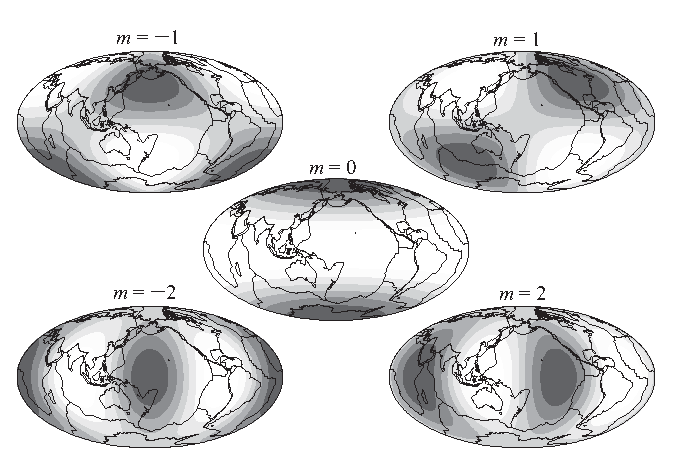
\includegraphics{../figures/appendixB/fig01.eps}
\end{center}
\caption[Real Y2m]{\label{fig:realY2}
五个实数表面球谐函数$\sY_{2\,-2},\sY_{2\,-1},\sY_{20},\sY_{21},\sY_{22}$。 阴影和非阴影区域分别对应正值和负值。单位球的整个表面用以~ $\phi=\pi$~为中心的~Aitoff~等面积投影显示。
格林威治子午线与边界椭圆重合。地球的海岸线和板块边界叠加在图上以供参考。}
\end{figure}
$2l+1$~个复表面球谐函数 $Y_{lm}(\theta,\phi)=X_{lm}(\theta)e^{im\phi}$,$-l\leq m\leq l$
为原子和分子角动量的量子理论中固有为复数的波函数提供了一组自然基。
另一方面,在许多地球物理应用中,我们希望将
固有为实数的场展开;这时更为方便的基包含~
$2l+1$~个实数函数~$\sqrt{2}X_{ll}(\theta)\cos l\phi,\ldots, X_{l0}(\theta),
\ldots,\sqrt{2}X_{ll}(\theta)\sin l\phi$。
我们保留~$-l\leq m\leq l$~这一的级数角标的范围,并以手书体字母来表示这些实数表面球谐函数:
\eq \label{B.realYdef}
\ylm(\theta,\phi)=\left\{\begin{array}{ll}
\sqrt{2}X_{l|m|}(\theta)\cos m\phi
& \mbox{if $-l\leq m<0$} \\
\vspace{-0.8 ex} & \vspace{-0.8 ex} \\
X_{l0}(\theta) & \mbox{if $m=0$} \\
\vspace{-0.8 ex} & \vspace{-0.8 ex} \\
\sqrt{2}X_{lm}(\theta)\sin m\phi
& \mbox{if $0<m\leq l$.}
\end{array}\right.
\en
\begin{figure}[!b]
\begin{center}
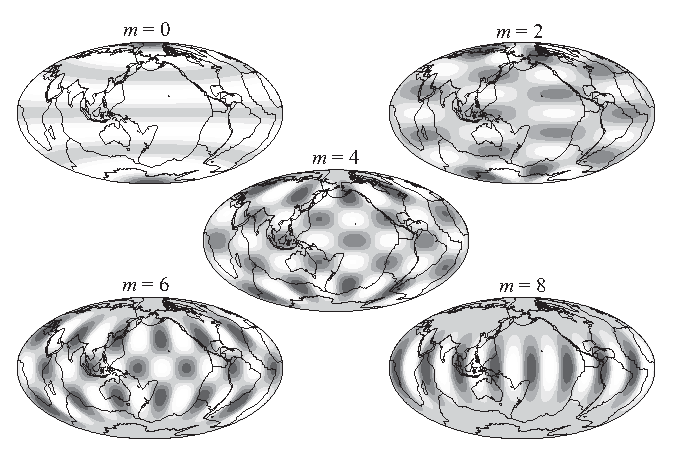
\includegraphics{../figures/appendixB/fig02.eps}
\end{center}
\caption[Real Y8m]{\label{fig:realY8}
五个偶数级数的实数表面球谐函数~$\sY_{80}$、$\sY_{82}$、$\sY_{84}$、 $\sY_{86}$、$\sY_{88}$。地图投影和其它信息
同图~\ref{fig:realY2}。}
\end{figure}
由~(\ref{B.realYdef})~定义的实数表面球谐函数~$\sY_{lm}$, 其中~$-l\leq m\leq l$,其正交意味着:
\eq \label{B.realnorm}
\int_\Omega \sY_{lm}\sY_{l'm'}\,d\Om=\delta_{ll'}\delta_{mm'}.
\en
此外,它们也满足实数球谐函数加法定理
\index{spherical-harmonic addition theorem}%
\eq \label{B.realaddth}
\sum_{m=-l}^l\sY_{lm}(\theta',\phi')\sY_{lm}(\theta,\phi)
=\left(\frac{2l+1}{4\pi}\right)P_l(\cos\Theta),
\en
其中$\cos\Theta=\cos\theta\cos\theta'+
\sin\theta\sin\theta'\cos(\phi-\phi')$。
贯穿本书,我们使用手书体字母所表示的实数球谐函数
~(\ref{B.realYdef})~作为实数基;球对称弹性和非弹性地球的本征函数分别在第~8~章和第~9.9~节中以~$\sY_{lm}$~表示,其中~$-l\leq m\leq l$。

零级实数球谐函数~$\sY_{l0}$~ 沿余纬度方向有~$l$~个结点,沿经度方向没有结点,因此被称为是{\em 带状\/}的,
\index{spherical harmonics!zonal}%
\index{zonal spherical harmonics}%
$\pm l$~级实数球谐函数~$\sY_{l\,\pm l}$~沿余纬度方向没有结点,沿经度方向有~ $2l$~个结点,被称为是{\em 条状\/}的。
\index{spherical harmonics!sectoral}%
\index{sectoral spherical harmonics}%
级数为~$-l<m<l$~的实数球谐函数~$\sY_{l\,\pm m}$~沿余纬度方向有~$l-|m|$~个结点,沿经度方向有~$2|m|$~个结点,被称为是{\em 网状\/}的。
\index{spherical harmonics!tesseral}%
\index{tesseral spherical harmonics}%
这种命名很容易记:条状球谐函数的正和负的区域形状就像一瓣瓣的橙子,
而网状球谐函数正负区域则像是网格化的单位球。
在图~\ref{fig:realY2}中,我们展示了五个次数为~2~的实数球谐函数~$\sY_{2\,-2}$, $\sY_{2\,-1}$、
$\sY_{20}$、$\sY_{21}$、 $\sY_{22}$,而图~\ref{fig:realY8},则展示了五个次数为~8~的偶数级数的球谐函数~$\sY_{80}$、$\sY_{82}$、
$\sY_{84}$、$\sY_{86}$、$\sY_{88}$。


%\section{Asymptotic Representation}
\section{渐近表达式}
\index{spherical harmonics!asymptotic representation|(}%
\label{B.sec.asym}

在~$l\gg 1$~极限下成立的~$X_{lm}(\theta)$~的渐近表达式可以通过将~JWKB~近似应用于其满足的微分方程~(\ref{eq:Legeqn2})~而得到。
\index{JWKB approximation}%
利用替换
\eq
X=(1-\mu^2)^{-1/2}Z,
\en
可以将勒让德方程转换为一维的薛定谔方程:
\eq
\ep^2\,\frac{d^{2\!}Z}{d\mu^2}+\left[\frac{a^2-\mu^2+\ep^2}
{(1-\mu^2)^2}\right]Z=0, \label{eq:JWKB}
\en
其中
\eq
\ep=\frac{1}{\sqrt{l(l+1)}},\qquad
a=\left[1-\frac{m^2}{l(l+1)}\right]^{1/2}.
\en
遵循~\textcite{brussaard&tolhoek57},我们寻求方程~(\ref{eq:JWKB})~在~$\ep\ll 1$~极限下具有以下形式的解
\eq \label{B.JWKBans}
Z=A\exp(i\ep^{-1}\psi).
\en
将~(\ref{B.JWKBans})~带入,并令~$\ep$~幂次相同的项相等,则从最低阶我们发现~
JWKB~相位~$\psi$~和振幅~$A$~分别满足{\em 程函方程\/}和{\em 输运方程\/}:
\index{eikonal equation}%
\index{transport equation}%
\eq
\left(\frac{d\psi}{d\mu}\right)^2\!\!-\frac{a^2-\mu^2}{(1-\mu^2)^2}=0,
\qquad \frac{d}{d\mu}\left(A^2\frac{d\psi}{d\mu}\right)=0.
\en
在我们感兴趣的区间~$-1\leq\mu\leq 1$~上有两个折返点~$\mu=\pm a$。
\index{turning point}%
对应的{\em 折返余纬度\/}
\index{turning colatitude}%
\index{colatitude!turning}%
分别位于北半球和南半球的~$\theta_0$~和~$\pi-\theta_0$~处,其中
\eq \label{B.turn}
\theta_0=\arcsin\left(\frac{|m|}{\sqrt{l(l+1)}}\right)\approx
\arcsin\left(\frac{|m|}{l+\half}\right).
\en
渐近解在内部区域~$\theta_0\ll\theta\ll\pi-\theta_0$~是振荡的,而在两个极区~ $0\leq\theta\ll\theta_0$~和~
$\pi-\theta_0\ll\theta\leq\pi$~则是瞬逝的。振荡解的形式为
\eqa \label{B.JWKBan2}
\lefteqn{X\approx C_+
(a^2-\mu^2)^{-1/4}\exp\left(i\ep^{-1}\int_0^{\mu}
\frac{\sqrt{a^2-\nu^2}}{1-\nu^2}d\nu\right)} \nonumber \\
&&\mbox{}+C_-(a^2-\mu^2)^{-1/4}\exp\left(-i\ep^{-1}\int_0^{\mu}
\frac{\sqrt{a^2-\nu^2}}{1-\nu^2}d\nu\right),
\ena
其中复数常数~$C_+$~和~$C_-$~为待定。
通过要求振荡解~(\ref{B.JWKBan2})~与瞬逝解在折返点~$\mu=\pm a$~处平滑连接,
并借助~JWKB~归一化条件~$\int_{-a}^aX^2\,d\/\mu
\approx 1/2\pi$,我们得到实数结果
\eq \label{eq:Xasym}
X\approx\frac{1}{\pi}
(a^2-\mu^2)^{-1/4}\cos\left[\ep^{-1}\int_0^{\mu}
\frac{\sqrt{a^2-\nu^2}}{1-\nu^2}d\nu-(l+m)\frac{\pi}{2}\right].
\en
(\ref{eq:Xasym})中的相位积分可以通过将被积函数改写为
\eq \label{B.twoterms}
\frac{\sqrt{a^2-\nu^2}}{1-\nu^2}=\frac{1}
{\sqrt{a^2-\nu^2}}-\frac{1-a^2}{(1-\nu^2)\sqrt{a^2-\nu^2}}.
\en
而进行解析计算。
(\ref{B.twoterms})~中的第一项的积分可以立即得到,而第二项的积分则需经过替换~ $\xi=\mu(a^2-\nu^2)^{1/2}$。
经一些整理,我们可以将次数为~$l$、级数为非负~($m\geq 0$)~的归一化
连带勒让德函数的渐近表达式写为
\eqa  \label{eq:Xlmasym} \lefteqn{
X_{lm}(\theta)\approx\frac{1}{\pi}
(\sin^{2\!}\theta-\sin^{2\!}\theta_0)^{-1/4}} \nonumber \\
&&\mbox{}
\times\cos\big[(l+\half)\arccos(\cos\theta/\!\cos\theta_0)\frac{}{}
\nonumber \\
&&\mbox{}
\qquad -m\arccos(\cot\theta/\!\cot\theta_0)
+m\pi-\quart\pi\big].\frac{}{}
\ena
\begin{figure}
\begin{center}
\scalebox{0.9}{
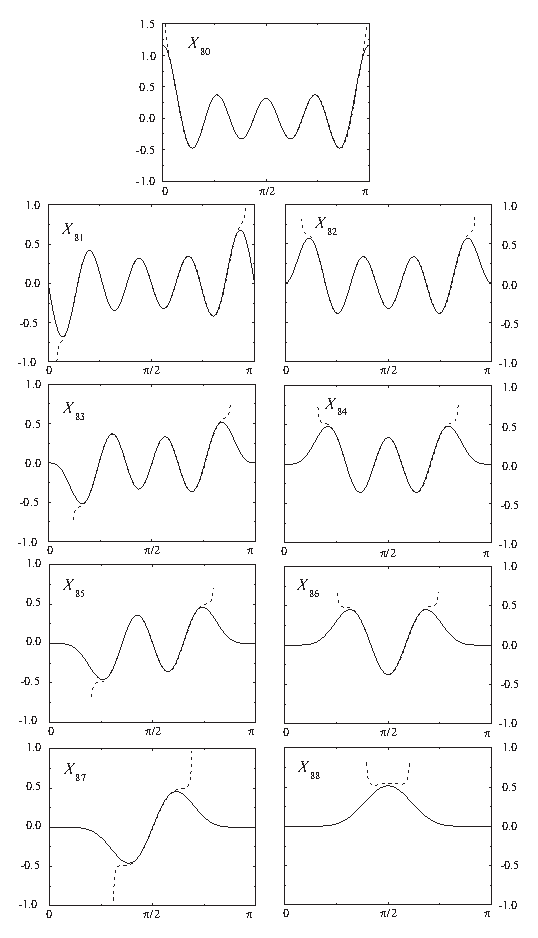
\includegraphics{../figures/appendixB/fig03.eps}
}
\end{center}
\caption[Asymp Xlm]{\label{figure:asymXlm}
精确~({\em 实线\/})~和渐近~({\em 虚线\/})~余纬球谐函数~ $X_{80}$、$X_{81}$、$X_{82}$、$X_{83}$、$X_{84}$、
$X_{85}$、$X_{86}$、$X_{87}$、$X_{88}$。当~$m\geq 0$~时,$X_{lm}$~很明显有~ $l-m$~个节点(参考图~\ref{fig:realY8})。除去~
$m=l$~的非振荡的情形,渐近近似式~(\ref{eq:Xlmasym})~在
折返余纬度~$\theta_0\ll
\theta\ll\pi-\theta_0$~之间能够准确地表示~$l\gg 1$~时的~$X_{lm}$。}
\end{figure}
级数为负数~$m<0$~的相应结果可以从对称关系~$X_{l\,-m}=(-1)^mX_{lm}$~得到。
图~\ref{figure:asymXlm}显示了~(\ref{eq:Xlmasym})~式在振荡区间~ $\theta_0\ll\theta\ll\pi-\theta_0$~内为精确的球谐函数~$X_{lm}$~提供了很好的近似,即使是~$l=8$~这种次数较低的。
在转折余纬度~$\theta_0$~和~$\pi-\theta_0$~处附近的发散是~JWKB~近似的一个特征;
用艾利函数所做的更完整的处理不仅可以分别得到瞬逝区间~$0\leq\theta\ll\theta_0$~和~$\pi-\theta_0\ll\theta\leq\pi$~内良好的渐近表达式,还能够较好地描述折返余纬度附近的过渡性表现~(Backus, Parker \& Constable \citeyear{backus&al96})。
 
在量子力学中,我们可以将渐近表达式
\eqa \label{eq:Ylmasym} \lefteqn{
Y_{lm}(\theta,\phi)\approx\frac{1}{\pi}
(\sin^{2\!}\theta-\sin^{2\!}\theta_0)^{-1/4}}
\nonumber \\
&&\mbox{}\times\cos\big[(l+\half)\arccos
(\cos\theta/\!\cos\theta_0)\frac{}{} \nonumber \\
&&\mbox{}\qquad -m\arccos(\cot\theta/\!\cot\theta_0)
+m\pi-\quart\pi\big]e^{im\phi}\frac{}{}
\ena
视为一个角动量为~$L=l+\half$~且~$L_z=m$~的在轨粒子的半经典波函数,如图~\ref{figure:Ylmasym}所示。

\begin{figure}[!b]
\begin{center}
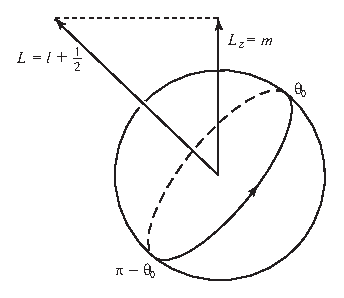
\includegraphics{../figures/appendixB/fig04.eps}
\end{center}
\caption[Ylm orbit]{\label{figure:Ylmasym}
一个在单位球面~$\Omega$~上南北半球折返余纬度~$\theta_0$~和~$\pi-\theta_0$~之间轨道上的量子力学粒子的半经典描述。角动量~${\bf L}$~的大小~$L=l+\textstyle{\frac{1}{2}}$~ 及其~$z$~分量长度~$L_z=m$~可以同时被确定。由于~$L_x$~和~$L_y$~是未定的,
其轨道必须被认为是以一种不确定的方式围绕着~$\hat{\bf z}$~轴在做“进动”。}
\end{figure}
两个赤道面上的分量~$L_x$~和~$L_y$~未被确定;因此,在~$\theta_0$~和~$\pi-\theta_0$~折返的所有大圆轨道对~$Y_{lm}$~有同样的贡献。
根据量子力学的对应原理,根据量子力学的对应原理,平方范数~$|Y_{lm}|^2\approx
(1/2\pi^2)(\sin^{2\!}\theta-\sin^{2\!} \theta_0)^{-1/2}$~是在~$\theta$~和~ $\theta+d\/\theta$~之间某一余纬度上找到该粒子的经典概率。

在~$m\ll l$~极限下,在振荡区间~$0\ll\theta\ll\pi$~内~(\ref{eq:Xlmasym})~式可以进一步简化为:
\eq \label{B.Xlpetitm}
X_{lm}(\theta)\approx\frac{1}{\pi}(\sin\theta)^{-1/2}
\cos\left[(l+\half)\theta+m\pi/2-\pi/4\right],
\en
同原来的相位积分表达式~(\ref{eq:Xasym})~一样,这一低阶的渐近近似对正负~$m$~都成立。
相应的复数表面球谐函数~$Y_{lm}(\theta,\phi)=X_{lm}(\theta)e^{im\phi}$~
可以被视为是高倾角、接近极轨道~($\theta_0\approx 0$和$\pi-\theta_0\approx\pi$)~ 上粒子的半经典波函数。
(\ref{B.Xlpetitm})~式中被忽略项的数量级为~$(l+\half)^{-1}$;
对于带状球谐函数~$m=0$~这一特例,展开式的下一项为~(Robin \citeyear{robin58}):
\eqa \label{B.Xlpetitm2}
\lefteqn{X_{l0}(\theta)\approx\frac{1}{\pi}(\sin\theta)^{-1/2}
\Big\{\!\cos\big[(l+\half)\theta-\pi/4\big]} \nonumber \\
&&\mbox{}+\eighth(l+\half)^{-1}\cot\theta
\sin\big[(l+\half)\theta-\pi/4\big]\Big\}.
\ena
在余纬度节点~$(l+\half)\theta\approx \threefourths\pi,\mbox{$\frac{7}{4}$}\pi,\ldots,(l-\fourth)\pi$,拓展关系式~(\ref{B.Xlpetitm2})~提供了一个更佳的近似。
\index{spherical harmonics!asymptotic representation|)}%

%\section{Spherical-Harmonic Expansions}
\section{球谐函数展开}
\index{spherical harmonics!expansion in|(}%
\label{section:exp}

令~$\psi(\theta,\phi)$~为单位球面上一个平方可积的复数函数,拥有{\em 拉普拉斯系数\/}
\index{Laplace coefficient}%
\eq
\psi_{lm}=\langle Y_{lm},\psi\rangle=\int_\Omega Y_{lm}^*\psi\,d\/\Om.
\label{eq:coeffic}
\en
我们来考虑一个用{\em 有限个\/}表面球谐函数的线性组合来近似~$\psi$~的问题,
以最小二乘的标准,我们试图找到系数~$\hat{\psi}_{lm}$,以满足
\eq \label{B.minimum}
\|\psi-\sum_{l=0}^L\sum_{m=-l}^l\hat{\psi}_{lm}Y_{lm}\|^2=
\mbox{极小}.
\en
利用正交归一性关系~(\ref{eq:ortho}),我们可以将~(\ref{B.minimum})~ 的左边写为以下形式
\eqa
\lefteqn{\|\psi-\sum_{l=0}^L\sum_{m=-l}^l\hat{\psi}_{lm}Y_{lm}\|^2=
\int_\Omega|\psi-\sum_{l=0}^L\sum_{m=-l}^l\hat{\psi}_{lm}Y_{lm}|^2\,d\/\Om}
\nonumber \\
&&\mbox{}=\|\psi\|^2+\sum_{l=0}^L
\sum_{m=-l}^l|\hat{\psi}_{lm}-\psi_{lm}|^2
-\sum_{l=0}^L\sum_{m=-l}^l|\psi_{lm}|^2.
\ena
很明显,这一分解在~$\hat{\psi}_{lm}=\psi_{lm}$~时有最小值。
因此,到第~$L$~次球谐函数的部分拉普拉斯求和
\eq
\psi_L=\sum_{l=0}^{L}\sum_{m=-l}^{l}\psi_{lm}Y_{lm},
\en
是在最小二乘法的意义上对~$\psi$~的最佳的有限球谐函数近似,它包含~$1+3+\cdots +(2L+1)=(L+1)^2$~项。该近似的平方误差为
\eq
\|\psi-\psi_L\|^2=\int_\Omega|\psi-\psi_L|^2\,d\/\Om
=\|\psi\|^2-\sum_{l=0}^{L}\sum_{m=-l}^{l}|\psi_{lm}|^2.
\en
可以证明,对于任一平方可积函数,我们能够让该截断误差要多小有多小: $\lim_{L\rightarrow\infty}\|\psi-\psi_L\|^2=0$。
\eq
而无限拉普拉斯求和
\psi=\sum_{l=0}^{\infty}\sum_{m=-l}^{l}\psi_{lm}Y_{lm}\quad
\mbox{其中}\quad\psi_{lm}=\int_{\Omega}Y_{lm}^*\psi\,d\/\Omega,
\label{eq:complex}
\en
则被称为{\em 平均收敛\/}。
\index{convergence in the mean}%
$\psi$~的平方范数是对展开系数平方的无限求和:
\eq \label{B.Parseval}
\|\psi\|^2=\int_{\Omega}|\psi|^2\,d\/\Omega=
\sum_{l=0}^{\infty}\sum_{m=-l}^l|\psi_{lm}|^2.
\en
(\ref{B.Parseval})~这一结果是球谐函数形式的{\em 帕塞瓦尔定理\/}。 
\index{Parseval's theorem}% 
归一化的内层求和
\eq \label{B.variance}
\sigma_l^2=\frac{1}{2l+1}\sum_{m=-l}^l|\psi_{lm}|^2
\en
是函数~$\psi$~在单位面积上单一次数~$l$~的方差或{\em 功率\/}。
\index{spherical harmonics!power spectrum}%
\index{spectrum!spherical harmonic}%
单位球上的狄拉克~delta~函数
\eq \label{B.Dirac}
(\sin\theta)^{-1}\delta(\theta-\theta')\delta(\phi-\phi')
=\sum_{l=0}^{\infty}\sum_{m=-l}^lY_{lm}^*(\theta',\phi')
Y_{lm}(\theta,\phi),
\en
对于所有~$l\geq 0$~都有{\em 平坦的\/}功率谱:$\sigma_l^2=1/4\pi$。
一个{\em 实数\/}函数~$\psi$~当然可以展开成~(\ref{eq:complex})~的形式;此时复数拉普拉斯系数满足~ $\psi_{l\,-m}=(-1)^m\psi_{lm}^*$。或者,更经济的做法是我们可以将~$\psi$~用实数表面球谐函数~(\ref{B.realYdef})~来展开:
\eq \label{B.realYexp}
\psi=\sum_{l=0}^{\infty}\sum_{m=-l}^{l}\Psi_{lm}\ylm\quad
\mbox{其中}\quad\Psi_{lm}=\int_{\Omega}\ylm\psi\,d\/\Omega.
\en
实数和复数展开系数~$\Psi_{lm}$~和~$\psi_{lm}$~之间有以下关系
\eq \label{B.Psipsi}
\Psi_{lm}=\left\{\begin{array}{ll}
\sqrt{2}\,\Re{\rm e}\,\psi_{l|m|}
& \mbox{若 $-l\leq m<0$} \\
\vspace{-0.8 ex} & \vspace{-0.8 ex} \\
\psi_{l0} & \mbox{若 $m=0$} \\
\vspace{-0.8 ex} & \vspace{-0.8 ex} \\
-\sqrt{2}\,\Im{\rm m}\,\psi_{lm}
& \mbox{若 $0<m\leq l$.}
\end{array}\right.
\en
在许多应用中,为方便起见,通常都避免负数级数,而将展开式~(\ref{B.realYexp})~写为较长但更易理解的形式:
\eq \label{B.abexp}
\psi=\sum_{l=0}^{\infty}
\left[\,a_{l0}X_{l0}+\sqrt{2}\sum_{m=1}^{l}X_{lm}
(a_{lm}\cos m\phi+b_{lm}\sin m\phi)\,\right],
\en
其中
\eq \label{B.abexp1}
a_{l0}=\int_{\Omega}X_{l0}\,\psi\,d\/\Omega,
\en
\eq
a_{lm}=\sqrt{2}\int_{\Omega}(X_{lm}\cos m\phi)\,
\psi\,d\/\Omega\quad\mbox{若 $1\leq m\leq l$},
\en
\eq \label{B.abexp2}
b_{lm}=\sqrt{2}\int_{\Omega}(X_{lm}\sin m\phi)\,
\psi\,d\/\Omega\quad\mbox{若 $1\leq m\leq l$}.
\en
实数场~(\ref{B.realYexp})~
或~(\ref{B.abexp})--(\ref{B.abexp2})~的帕塞瓦尔定理~(\ref{B.Parseval})~为
\eq
\|\psi\|^2=\sum_{l=0}^{\infty}\sum_{m=-l}^l\Psi_{lm}^2
=\sum_{l=0}^{\infty}\left[a_{l0}^2+
\sum_{m=1}^l(a_{lm}^2+b_{lm}^2)\right].
\en
该展开式在单位面积上单一次数~$l$~的功率为
\index{spherical harmonics!power spectrum}%
\index{spectrum!spherical harmonic}%
\eq \label{B.variance2}
\sigma_l^2=\frac{1}{2l+1}\sum_{m=-l}^l\Psi_{lm}^2=
\frac{1}{2l+1}\left[a_{l0}^2+
\sum_{m=1}^l(a_{lm}^2+b_{lm}^2)\right].
\en
上述所有讨论适用于单位球面~$\Omega$~上的场~$\psi(\theta,\phi)$。 
三维场~$\psi(\br)$~可以用球谐函数~$Y_{lm}$、
$\ylm$~或~$\sqrt{2}\,X_{ll}\cos l\phi,\ldots,
X_{l0},\ldots,X_{ll}\sin l\phi$~展开,
只要让系数~$\psi_{lm}$、$\Psi_{lm}$~或~
$a_{l0}$、$a_{lm}$、$b_{lm}$~是半径~$r$~的函数即可。

大地测量学所使用的标准惯例与~(\ref{B.abexp})--(\ref{B.abexp2})~相似,
只是奇数~$m$~的实数球谐函数的符号不同,且平方范数为~$4\pi$~而不是~1~ (Lambeck \citeyear{lambeck88};
Stacey \citeyear{stacey92})。
此时一个实数场的展开式为:
\eq \label{B.geodesy}
\psi=\sum_{l=0}^{\infty}\sum_{m=0}^{l}
p_{lm}(c_{lm}\cos m\phi+
s_{lm}\sin m\phi),
\en
其中~$p_{lm}=\sqrt{4\pi}\,(2-\delta_{m0})(-1)^mX_{lm}$。 
大地测量学中的展开系数与~(\ref{B.abexp1})--(\ref{B.abexp2})~中的系数之间的关系为
\eq
c_{lm}=\sqrt{4\pi}\,(-1)^ma_{lm},\qquad
s_{lm}=\sqrt{4\pi}\,(-1)^mb_{lm}.
\en
地磁学中经常用到的所谓准归一化~Schmidt~球谐函数与~$X_{lm}$和$p_{lm}$~ 都不一样~(Chapman \& Bartels \citeyear{chapman&bartels40};
Backus, Parker \& Constable \citeyear{backus&al96})。
地球物理学界的一个琐碎却难以逃避的烦恼是,球谐函数的符号和归一化
惯例在不同的学科(甚至不同的研究)之间都有所不同,因此在比较或使用其结果时必须十分小心。 在这方面量子力学并不那么巴尔干化,\textcite{condon&shortley35}~和 \textcite{edmonds60}~中的复数球谐函数~$Y_{lm},-l\leq m\leq l$~ 已经几乎是通用的了。
\index{spherical harmonics!expansion in|)}%

%\section{Integration Around a Great Circle}
\section{绕大圆弧的积分}
\label{section:B.9}

我们根据单位球面~$\Omega$~上以右手法则定义的{\em 正极点\/}~$\bar{\br}$~来指定一个{\em 定向大圆路径\/},
\index{great-circular average}%
\index{positive pole}%
\index{pole!positive}%
如果该路径是依序连接~$\brh_1$~和~$\brh_2$~两点的测地线小圆弧的延伸,如图~\ref{B.fig:gtcirc}~所示,
则$\bar{\br}=(\brh_1\times\brh_2)/
\|\brh_1\times\brh_2\|$。
\begin{figure}[!b]
\begin{center}
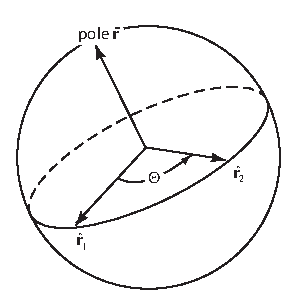
\includegraphics{../figures/appendixB/fig05.eps}
\end{center}
\caption[GC Pole]{\label{B.fig:gtcirc}
一个依次通过$\hat{\bf r}_1$~和~$\hat{\bf r}_2$~两点的定向大圆路径的极点~$\overline{\bf r}=(\hat{\bf r}_1\times\hat{\bf r}_2)
/\|\hat{\bf r}_1\times\hat{\bf r}_2\|$。
反向大圆弧的极点是对跖点~$-\bar{\bf r}$。}
\end{figure}
该大圆弧极点的球极坐标~$\bar{\theta},\bar{\phi}$~可以用“源点"和”接收点"坐标~$\theta_1,\phi_1$~和~$\theta_2,\phi_2$~表示为:
\eq \label{B.poledef1}
\cos\bar{\theta}=\frac{\sin\theta_2\sin\theta_1\sin(\phi_2-\phi_1)}
{\sin\Theta},
\en
\eq
\label{B.poledef2}
\tan\bar{\phi}=\frac{\sin\theta_2\cos\theta_1\cos\phi_2
-\cos\theta_2\sin\theta_1\cos\phi_1}
{\cos\theta_2\sin\theta_1\sin\phi_1
-\sin\theta_2\cos\theta_1\sin\phi_2},
\en
其中~$\cos\Theta=\brh_1\cdot\brh_2=
\cos\theta_2\cos\theta_1+\sin\theta_2
\sin\theta_1\cos(\phi_2-\phi_1)$。

一个函数~$\psi(\theta,\phi)$~的{\em 大圆平均\/}的定义为
\index{great-circular average}%
\eq \label{B.gtcircave}
\bar{\psi}(\bar{\theta},\bar{\phi})=\frac{1}{2\pi}
\oint_{\,\bar{\theta},\bar{\phi}}
\psi(\theta,\phi)\,d\/\Delta,
\en
其中积分是在整个圆周上进行,$d\/\Delta$~为微分角弧长。
我们可以将~$\bar{\psi}$~视为单位球上位置的一个连续函数,它是通过对所有可能的定向大圆积分并将平均值赋予极点。由于绕大圆的积分方向无关紧要,我们一定会得到
\eq \label{B.psibareven}
\bar{\psi}
(\pi-\bar{\theta},\bar{\phi}+\pi)=
\bar{\psi}(\bar{\theta},\bar{\phi}),
\en
也就是说,任何场~$\psi$~的大圆平均~$\bar{\psi}$~一定是~$\Omega$~上位置~$\bar{\bf r}$~的{\em 偶函数\/}。
\index{even function}%

次数为~$l$~的表面球谐函数的大圆平均为
\eq \label{B.Ylmoint}
\frac{1}{2\pi}\oint_{\,\bar{\theta},\bar{\phi}}
Y_{l}(\theta,\phi)\,d\/\Delta=P_l(0)Y_{l}(\bar{\theta},\bar{\phi}).
\en
这一异常简单的结果,可以遵循~Roberts \& Ursell (\citeyear{roberts&ursell60})~通过考虑一个~
$\bzh$轴通过极点$\bar{\theta},\bar{\phi}$~的球极坐标系来证明。
函数~$Y_l(\bar{\theta},\bar{\phi})$~在
该坐标系中可以写为球谐函数基~$Y_{lm}$~的线性组合,这里~$-l\leq m\leq l$。
带状球谐函数~$Y_{l0}$~满足~(\ref{B.Ylmoint})~式,两边的值均为~
$\sqrt{(2l+1)/4\pi}\,P_l(0)$,所有非带状球谐函数也满足它,但两边的值
为零。因此,(\ref{B.Ylmoint})~对一般的实数或复数球谐函数~ $Y_l$~都是成立的。
在附录~C.8~中,我们利用由~Backus (\citeyear{backus64})~率先提出的一个更一般的推导,来为此大圆等式提供另一个证明。
后一个推导同时还提供了一个计算~$\theta_1,\phi_1$~和~$\theta_2,\phi_2$~两点 之间的小圆弧积分的方法。

$\bar{\psi}(\bar{\theta},\bar{\phi})$~的球谐函数展开系数~ $\bar{\psi}_{lm}$~与平均后函数~$\psi(\theta,\phi)$~的系数~ $\psi_{lm}$~存在以下关系:
\eq \label{B.psibarlm}
\bar{\psi}_{lm}=P_l(0)\,\psi_{lm}.
\en
勒让德多项式$P_l(0)$的显式表达式为
\eq \label{B.Plzero}
P_l(0)=\left\{\begin{array}{ll}
0 & \mbox{$l$ 为奇数} \\
\vspace{-0.8 ex} & \vspace{-0.8 ex} \\
(-1)^{l/2}\,l!\,2^{-l}[(l/2)!]^{-2} & \mbox{$l$ 为偶数.}
\end{array}\right.
\en
不存在任何奇数次的系数~$\bar{\psi}_{lm}$~与对~(\ref{B.psibareven})~的简单观察是一致的。
基本上,由于大圆路径上对跖点~$\pm\brh$~的抵消作用,任何奇数次球谐函数的积分为零。对偶数高次数的渐近极限~$P_l(0)\rightarrow (-1)^{l/2}\sqrt{2/\pi l}$~表明大圆积分是一个平滑过程:如果~$\psi$~的功率谱~$\sigma_l^2$~以~ $l^{-\alpha}$~的形式衰减,那么~$\bar{\psi}$~的功率谱就会以~ $l^{-\alpha-1}$~的形式衰减。(\ref{B.Ylmoint})~式适用于实数球谐函数~(\ref{B.realYdef}),因而~(\ref{B.psibarlm})~对相关的系数$\bar{\Psi}_{lm}$~和~
$\Psi_{lm}$~是成立的。表~B.2~列出了当~$l=0,2,4,6,\ldots$时$P_l(0)$~的值。
\begin{table}[!t]
\centering
\begin{tabular}{|c|c|} \hline
& \\
次数~$l$~&~$P_l(0)$~值
& \\ \hline
& \\
0 & 1 \\
\vspace{-1.0 ex} & \vspace{-1.0 ex} \\
2 & $-1/2$ \\
\vspace{-1.0 ex} & \vspace{-1.0 ex} \\
4 & 3/8 \\
\vspace{-1.0 ex} & \vspace{-1.0 ex} \\
6 & $-5/16$ \\
\vspace{-1.0 ex} & \vspace{-1.0 ex} \\
\vdots & \\
\vspace{-1.0 ex} & \vspace{-1.0 ex} \\
$\infty$ & $(-1)^{l/2}\sqrt{2/\pi l}$ \\
& \\ \hline
\end{tabular}
\caption[table:Plzero]
{次数$l$为偶数的大圆平均滤波系数~$P_l(0)$~的数值。$l\rightarrow\infty$~时的极限是用~Stirling~公式来近似~(\ref{B.Plzero})~中的阶乘而得到的渐近表达式。}
\end{table}

%\section{Practical Considerations}
\section{实际上的考量}
\index{spherical harmonics!practical considerations|(}%

计算表面球谐函数的最佳程序取决于具体的应用。
要在一个球对称地球上合成简正模式地震图,我们只需要连带勒让德函数~ $P_{l0}$、$P_{l1}$、
$P_{l2}$~和它们的余纬度导数。这些可以利用固定级数的递推关系~(\ref{eq:stable})~来计算,这样在次数~$l$~递增的方向上迭代是稳定的。
为了使端点~$\mu=\pm1$~附近的误差最小,并得到在~$-1\leq\mu\leq 1$~区间内一致成立的结果,定义一个辅助函数~$R_{lm}$~是有益的:
\eq
P_{lm}(\mu)=(1-\mu^2)^{m/2}R_{lm}(\mu).
\en
这样,以下预处理的递推关系
\eq \label{B.Rrecur}
(l-m+1)R_{l+1\,m}-(2l+1)\mu R_{lm}+(l+m)R_{l-1\,m}=0
\en
的初始值为$R_{00}=1$、$R_{10}=\mu$、$R_{11}=1$、$R_{21}=3\mu$
和$R_{22}=3$、$R_{32}=15\mu$。
导数$dP_{l0}(\cos\theta)/d\theta$、$dP_{l1}(\cos\theta)/d\theta$
和$dP_{l2}(\cos\theta)/d\theta$可以从~(\ref{B.dPdmu})中的第二个或第四个等式得到:
\eqa \lefteqn{
\frac{dP_{lm}}{d\theta}=-m\cot\theta\,P_{lm}
+(l+m)(l-m+1)P_{l\,m-1}} \nonumber \\
&&\mbox{}\hspace{1.5 mm}=l\cot\theta\,P_{lm}
-(l+m)\,{\rm csc}\,\theta\,P_{l-1\,m}.
\ena
(\ref{B.Rrecur})~的每次迭代其舍入误差都会乘以一个数量级为~1~的因子,
因而需要的结果可以精确地计算到非常高的次数,而不会有明显的精度损失。

要计算非球对称地球上的实数或复数的源点和接收点矢量,我们需要所有级数 的~$X_{lm}$~和~$dX_{lm}/d\/\theta$。此时最简单的方法是利用固定次数的递推关系~(\ref{B.Libb1}),它在级数$m$递减的方向递推结果是稳定的。
定义一个辅助函数~$W_{lm}$~为:
\eq
X_{lm}=(\sin\theta)^mW_{lm},
\en
我们可以将该关系写为如下预处理形式
\eqa \label{B.Libbrecur} \lefteqn{
(1-\mu^2)\sqrt{(l-m)(l+m+1)}\,W_{l\,m+1}+2m\mu W_{lm}}
\nonumber \\
&&\mbox{}+\sqrt{(l+m)(l-m+1)}\,W_{l\,m-1}=0,
\ena
其中$\mu=\cos\theta$。(\ref{B.Libbrecur})的初始值为
\eq
W_{ll}=(-1)^l\left(\frac{2l+1}{4\pi}\right)^{\!1/2}
\frac{\sqrt{(2l)!}}{2^ll!},\qquad
W_{l\,l-1}=-\sqrt{2l}\,\mu W_{ll}.
\en
要注意的是,没有必要将递推进行到~$m=0$~以下;级数为负数的可以用对称性~ $X_{l\,-m}=(-1)^{l+m}X_{lm}$~得到。
在~$m=l$~附近,每次迭代的舍入误差都会乘上一个数量级为~$\sqrt{l}$~的因子;正因如此,即便在~(\ref{B.Libbrecur})~的计算中用双精度,也只能提供令人满意的结果到次数~$l\approx 200$。
Libbrecht (\citeyear{libbrecht85})~介绍了一个基于级数和次数均可变的递推关系~(\ref{B.Libb2})~的稍微复杂一点的方法,必要的话可以用来计算更高次数的球谐函数~$X_{lm}$。
余纬度导数~$dX_{lm}/d\/\theta$~可以用下式计算:
\eqa
\lefteqn{\frac{dX_{lm}}{d\/\theta}=\half\sqrt{(l-m)(l+m+1)}\,X_{l\,m+1}}
\label{eq:Xrecur1} \nonumber \\
&&\mbox{}-\half\sqrt{(l+m)(l-m+1)}\,X_{l\,m-1},
\ena
它是~(\ref{B.dPdmu})~中前两个等式合并和修改的结果。

Masters \& Richards-Dinger (\citeyear{masters&dinger98})~提出了另一种方法,能够同时计算~$X_{lm}$~和~ $dX_{lm}/d\/\theta$。他们将~(\ref{B.dPdmu})~中的前两个等式改写为一对耦合的递推关系:
\eq \label{B.dinger1}
X_{l\,m-1}=-\frac{dX_{lm}/d\theta+m\cot\theta X_{lm}}
{\sqrt{(l+m)(l-m+1)}},
\en
\eqa \label{B.dinger2} \lefteqn{
\frac{dX_{l\,m-1}}{d\theta}=(m-1)\cot\theta
X_{l\,m-1}} \nonumber \\
&&\mbox{}+\sqrt{(l+m)(l-m+1)}\,X_{lm}.
\ena
稳定的迭代方向同样是从~$m=l$~递减到~$m=0$;此时的初始值为
\eqa \label{B.dinger3} \lefteqn{
X_{ll}=(-1)^l\left(\frac{2l+1}{4\pi}\right)^{\!1/2}
\frac{\sqrt{(2l)!}}{2^ll!}\,(\sin\theta)^l,\qquad
\frac{dX_{ll}}{d\theta}=l\cot\theta X_{ll}.} \nonumber \\
&&\mbox{}
\ena
由于没有做任何预处理,在次数较大~$l\gg 1$~时,(\ref{B.dinger3})~在极点余纬度附近~$\theta\approx 0$~或~ $\theta\approx\pi$~会出现下溢。
在这种情况下,他们通过用$X_{ll}=(-1)^l$作为迭代初始值来确定
符号,并在递减到~$m=0$~的递推过程中将~$X_{lm}$~及其导数~$dX_{lm}/d\theta$~进行缩放,以避免溢出。
在计算结束时,再将这种缩放除去,并容许下溢发生;
对最终的结果做归一化,使其与球谐函数的加法定理相符:
\eq \label{B.guynorm}
\sum_{m=-l}^lX_{lm}^2=(2l+1)/4\pi.
\en
\index{spherical harmonics!practical considerations|)}%

%\section{Complex Legendre Functions}
\section{复数勒让德函数}
\index{Legendre function!complex|(}%
\index{complex Legendre function|(}%
\label{sec:travel}

勒让德多项式~$P_l(\mu)$~和连带勒让德函数~$P_{lm}(\mu)$~的
定义可以做相当的拓展,容许所有的三个参数~$l,m$~和~$\mu$~ 均为复数。在本书中我们不需要这样做;
全面性的讨论请见~Erd\'{e}lyi, Magnus, Oberhettinger \& Tricomi
(\citeyear{erdelyi&al53})~和~Robin (\citeyear{robin58})。在单位球面上行波的分析中会遇到次数~$\lambda$~为复数、级数为非负整数~$m=0,1,2,\ldots$~和自变量为~$-1\leq\mu\leq 1$~的实数的勒让德函数;
我们在此对这些地震学中使用的函数的重要特性做一个概述。

%\subsection{Legendre functions of the first and second kind}
\subsection{第一类和第二类勒让德函数}
\index{Legendre function!of the first kind|(}%
\index{Legendre function!of the second kind|(}%

我们在第~11~章和第~12~章对面波和体波格林函数张量的分析中使用了算子系统,
使我们能够避免明确地考虑级数~$m\not=0$~的情况。
因此,我们首先考虑方位上对称的级数为~$m=0$~的函数。
由于勒让德方程
\eq \label{B.compLeg}
(1-\mu^2)\frac{d^2\!X}{d\mu^2}-2\mu\frac{dX}{d\mu}+\lambda(\lambda+1)X=0
\en
是二阶的,它有两个线性独立解,通常以~$P_{\lambda}$~和~ $Q_{\lambda}$~来表示,分别称为{\em 第一类和第二类勒让德函数\/}。鉴于我们的目的,将它们以积分表达式来定义最为方便
\eq \label{B.Plambda}
P_{\lambda}(\mu)=\frac{2}{\pi}\,\Im{\rm m}\int_0^{\infty}
\left(\mu-i\sqrt{1-\mu^2}\cosh t\right)^{-\lambda-1}\,dt,
\en
\eq \label{B.Qlambda}
Q_{\lambda}(\mu)=\Re{\rm e}\int_0^{\infty}
\left(\mu-i\sqrt{1-\mu^2}\cosh t\right)^{-\lambda-1}\,dt,
\en
该式在~$\Re{\rm e}\,\lambda>-1$~时成立。
通过选择被积函数中乘方的主值,可以使~$P_{\lambda}$~和~ $Q_{\lambda}$~均为单值函数。 

第一类勒让德函数与非负整数次数~$\lambda=0,1,\ldots$~的勒让德多项式~(\ref{B.Legpoldef})~相同。
而相应的第二类勒让德函数~$Q_0, Q_1,\ldots$~可以表示为
\eq \label{Qsubldef}
Q_l(\mu)=\half P_l(\mu)\ln\left(\frac{1+\mu}{1-\mu}\right)
-M_{l-1},
\en
其中~$M_{-1}=0$,而当~$l>0$~时
\eq
M_{l-1}=\frac{2l-1}{1(l-0)}\,P_{l-1}+\frac{2l-5}{3(l-1)}
\,P_{l-3}+\frac{2l-9}{5(l-2)}\,P_{l-5}+\cdots.
\en
在端点~$\mu=\pm 1$~处的对数奇点是所有复数次数的~$Q_{\lambda}$~的特性,而不仅仅是对~$\lambda=0,1,\ldots$;
当~$\lambda\neq 0,\pm 1,\ldots$~时,$P_\lambda$~在~$\mu=-1$~ 处有单一的对数奇点。
(\ref{B.Plambda})--(\ref{B.Qlambda})~两式向~$\Re{\rm e}\,\lambda\leq -1$~区域的解析延拓满足对称关系
\eq \label{B.PQnegl}
P_{-\lambda-1}=P_{\lambda},\qquad
Q_{-\lambda-1}=Q_{\lambda}-\pi\cot\lambda\pi\,P_{\lambda}.
\en
(\ref{B.PQnegl})~中的第二个公式表明,$Q_{\lambda}$~在每个负整数~ $\lambda=-1,-2,\ldots$~处都有一个简单极点。
自变量为正负的勒让德函数的值具有以下关系
\eq \label{B.Pnegmu}
P_{\lambda}(-\mu)=\cos\lambda\pi\,P_{\lambda}(\mu)-
\frac{2}{\pi}\sin\lambda\pi\,Q_{\lambda}(\mu),
\en
\eq \label{B.Qnegmu}
Q_{\lambda}(-\mu)=-\cos\lambda\pi\,Q_{\lambda}(\mu)-
\frac{\pi}{2}\sin\lambda\pi\,P_{\lambda}(\mu).
\en
\index{Legendre function!of the first kind|)}%
\index{Legendre function!of the second kind|)}%

%\subsection{Travelling-wave Legendre functions}
\subsection{行波勒让德函数}
\index{Legendre function!travelling-wave|(}%
\index{travelling-wave Legendre function|(}%

本书中使用的{\em 行波勒让德函数\/}是~Nussenzveig (\citeyear{nussenzveig65})~中所描述的:
\eq \label{B.Q12def}
Q_{\lambda}^{(1,2)}=\half\left(P_{\lambda}\pm\frac{2i}{\pi}Q_{\lambda}\right),
\en
其中左右两边的双重上角标分别对应于右边的上下双重符号。
当~$\Re{\rm e}\,\lambda >-1$~时,我们有显式积分表达式
\eq \label{B.Q12int}
Q_{\lambda}^{(1,2)}(\mu)=\pm\frac{i}{\pi}\int_0^{\infty}
\left(\mu\pm i\sqrt{1-\mu^2}\cosh t\right)^{-\lambda-1}\,dt.
\en
从~(\ref{B.PQnegl})--(\ref{B.Qnegmu})~以及定义~(\ref{B.Q12def}),我们发现
\eq \label{B.Q12negl}
Q_{-\lambda-1}^{(1,2)}=Q_{\lambda}^{(1,2)}\mp i\cot\lambda\pi\,P_{\lambda},
\en
\eq \label{B.Q12negmu}
Q_{\lambda}^{(1,2)}(-\mu)=e^{\mp i\lambda\pi}Q_{\lambda}^{(2,1)}(\mu).
\en
$Q_{\lambda}^{(1)}$~和~$Q_{\lambda}^{(2)}$~这两个行进波勒让德函数均在
负整数~$\lambda=-1,-2,\ldots$~处有简单极点,这些极点在两者相加后抵消,、而形成第一类勒让德函数~$P_{\lambda}$。
综合上述次数和自变量替换~$\lambda\rightarrow -\lambda-1$~和~$\mu\rightarrow -\mu$~的结果,我们可以得到不同类型勒让德函数之间的其它关系,例如:
\eq
P_{\lambda}(-\mu)=e^{\mp i\lambda\pi}P_{\lambda}(\mu)
\pm 2i\sin\lambda\pi\,Q_{\lambda}^{(1,2)}(\mu)
\label{eq:PQrel}
\en
和
\eqa \label{B.JEROEN} \lefteqn{
Q_{-\lambda-1}^{(1,2)}(\mu)=
-e^{\pm 2i\lambda\pi}Q_{\lambda}^{(1,2)}(\mu)} \nonumber \\
&&\mbox{}
\pm ie^{\pm i\lambda\pi}\tan(\lambda+\half)\pi\,
P_{\lambda}(-\mu).
\ena
我们用~(\ref{B.JEROEN})~式将球对称地球的行波格林函数
张量表示为~(\ref{eq:11.repre3})~这一最容易解释的形式。

四种勒让德函数在复数次数~$|\lambda|\gg 1$~的极限下的渐近表达式为
\eq
P_{\lambda-\subhalf}(\cos\theta)\approx
\left(\frac{2}{\pi\lambda\sin\theta}
\right)^{1/2}\cos(\lambda\theta-\pi/4),
\label{B.Plmasym}
\en
\eq
Q_{\lambda-\subhalf}(\cos\theta)\approx-
\left(\frac{\pi}{2\lambda\sin\theta}
\right)^{1/2}\sin(\lambda\theta-\pi/4),
\label{B.Qlmasym}
\en
\eq
Q_{\lambda-\subhalf}^{(1,2)}(\cos\theta)\approx
\left(\frac{1}{2\pi\lambda\sin\theta}
\right)^{1/2}\exp\left[\mp i(\lambda\theta-\pi/4)\right].
\label{B.Q12masym}
\en
(\ref{B.Plmasym})--(\ref{B.Q12masym})~式在振荡区间~$0\ll\theta\ll\pi$~ 和~$|{\rm arg}\,\lambda|\ll\pi$~的扇形区域内处处成立。
很明显,$P_{\lambda}$~和~$Q_{\lambda}$~表示余纬度驻波,而~ $Q_{\lambda}^{(1)}$~和~$Q_{\lambda}^{(2)}$~则分别表示在~$\theta$~增大和减小的方向上传播的行波。
\index{Legendre function!travelling-wave|)}%
\index{travelling-wave Legendre function|)}%

%\subsection{Associated Legendre functions}
\subsection{连带勒让德函数}
\index{associated Legendre function|(}%
\index{Legendre function!associated|(}%

正整数级数~$m=1,2,\ldots$~的{\em 连带勒让德函数\/}可以类比~(\ref{B.PlmPl})~式定义为:
\eq \label{B.PlamPlam}
P_{\lambda m}(\mu)=(1-\mu^2)^{m/2}
\left(\frac{d}{d\mu}\right)^m
P_{\lambda}(\mu),
\en
\eq \label{B.QlamQlam}
Q_{\lambda m}(\mu)=(1-\mu^2)^{m/2}
\left(\frac{d}{d\mu}\right)^m
Q_{\lambda}(\mu).
\en
而类比~(\ref{B.Q12def})~式,连带行波勒让德函数为:
\eq \label{B.Q12lamdef}
Q_{\lambda m}^{(1,2)}=\half\left(P_{\lambda m}
\pm\frac{2i}{\pi}Q_{\lambda m}\right).
\en
显然,我们也可以用~$Q^{(1,2)}_{\lambda}$~将~$Q^{(1,2)}_{\lambda m}$~表示为:
\eq \label{B.TlamTlam}
Q^{(1,2)}_{\lambda m}(\mu)=(1-\mu^2)^{m/2}
\left(\frac{d}{d\mu}\right)^mQ^{(1,2)}_{\lambda}(\mu).
\en
(\ref{B.Q12lamdef})~中左、右半平面的函数可以由推广的~(\ref{B.JEROEN})~式联系起来:
\eqa \label{B.JEROEN2} \lefteqn{
Q_{-\lambda-1\,m}^{(1,2)}(\mu)=
-e^{\pm 2i\lambda\pi}Q_{\lambda m}^{(1,2)}(\mu)} \nonumber \\
&&\mbox{}
\pm i(-1)^me^{\pm i\lambda\pi}\tan(\lambda+\half)\pi\,
P_{\lambda m}(-\mu).
\ena
(\ref{B.JEROEN2})~式被用于行波矩张量响应~(\ref{eq:11.acctrave})~的推导中。四种连带勒让德函数的渐近表达式为
\eqa \lefteqn{
P_{\lambda-\subhalf\,m}(\cos\theta)\approx(-\lambda)^m
\left(\frac{2}{\pi\lambda\sin\theta}
\right)^{1/2}} \nonumber \\
&&\mbox{}\times\cos(\lambda\theta+m\pi/2-\pi/4),\frac{}{}
\label{B.Plammasym}
\ena
\eqa \lefteqn{
Q_{\lambda-\subhalf\,m}(\cos\theta)\approx-(-\lambda)^m
\left(\frac{\pi}{2\lambda\sin\theta}
\right)^{1/2}} \nonumber \\
&&\mbox{}\times\sin(\lambda\theta+m\pi/2-\pi/4),\frac{}{}
\label{B.Qlammasym}
\ena
\eqa \lefteqn{
Q_{\lambda-\subhalf\,m}^{(1,2)}(\cos\theta)\approx(-\lambda)^m
\left(\frac{1}{2\pi\lambda\sin\theta}
\right)^{1/2}} \nonumber \\
&&\mbox{}\times\exp\left[\mp i(\lambda\theta+m\pi/2-\pi/4)\right].\frac{}{}
\label{B.Q12lamasym}
\ena
以上结果在~$|\lambda|\gg 1$~的极限下当级数为{\em 小的\/}正整数~$m=1,2,\ldots$~时成立。
Clemmow (\citeyear{clemmow61}),
Burridge (\citeyear{burridge66})~和~Ansell (\citeyear{ansell73})~ 中讨论了这两个行波勒让德函数的另一种定义,其中保持了~$\exp[\mp i(\lambda\theta+m\pi/2-\pi/4)]$~这一根本的渐近特征。
\index{associated Legendre function|)}%
\index{Legendre function!associated|)}%
\index{Legendre function!complex|)}%
\index{complex Legendre function|)}%

%\section{Vector Spherical Harmonics}
\section{矢量球谐函数}
\index{spherical harmonics!vector|(}%
\index{vector spherical harmonics|(}%
\label{section:tv}

到目前为止,我们只考虑了标量场~$\psi$~的表面球谐函数中展开。
在本中,我们讨论将矢量场~$\bu$~用{\em 矢量球谐函数\/}展开的问题。为具体化起见,我们
假定~$\bu$~为实数的,并用实数的标量球谐函数~$\ylm$, $-l\leq m\leq l$,来定义\textcolor{red}{矢量}球谐函数;
然而,以类比的方式,完全可以用~$Y_{lm}$, $-l\leq m\leq l$,来定义复数的矢量球谐函数。
在附录~C~中,我们将考虑用复数广义球谐函数来展开矢量和更高阶的张量场。

%\subsection{Helmholtz representation of a tangent vector}
\subsection{切向矢量的亥姆霍兹表示}
\index{Helmholtz representation|(}%
\index{tangent vector|(}%
\index{vector!tangent|(}%

基本思路是用三个标量场来表示~$\bu$,且每一个标量场都用~$\ylm$, $-l\leq m\leq l$~来展开。
一个明显的出发点是~$\bu=u_r\brh+u_\theta\bthetah+u_\phi\bphih$~这一三分量形式;然而,它有一个不好的特性,在极点~$\theta=0$~和~ $\theta=\pi$~处为奇点。一个更有效的方法
是基于将切向矢量场~$\bu^{\Omega}=\bu-u_r\brh$~写为表面梯度和表面旋度之和的{\em 亥姆霍兹表示\/}:
\eq \label{B.Helm}
\bu^{\Omega}=\bdel_1V-\brh\times\bdel_1W,
\en
其中
\eq \label{B.Helm2}
\int_{\Omega}V\,d\/\Om=\int_{\Omega}W\,d\/\Om=0.
\en
对于单位球面~$\Omega$~上的任一切向矢量~$\bu^{\Omega}$,存在唯一的一组标量场~$V$~和~$W$,既满足~(\ref{B.Helm})~式,且在~(\ref{B.Helm2})~式的意义上平均值为零。(\ref{B.Helm})~式中的表面旋度项负号的引入是为了便于与较早的矢量球谐函数的惯例相一致~(Morse \& Feshbach \citeyear{morse&feshbach53})。

在~(\ref{B.Helm})~式两边点乘算子~$\bdel_1$~和~$\brh\times\bdel_1$,
并利用关系式~$\bdel_1\cdot\bdel_1
=(\brh\times\bdel_1)\cdot(\brh\times\bdel_1)=
\del_1^2$和$\bdel_1\cdot(\brh\times\bdel_1)=
(\brh\times\bdel_1)\cdot\bdel_1=0$,我们得到解耦的方程
\eq \label{B.Helm3}
\del_1^2V=\bdel_1\cdot\bu^{\Omega},\qquad\del_1^2W
=-(\brh\times\bdel_1)\cdot\bu^{\Omega}.
\en
要利用这些方程来得到标量场~$V$~和~$W$,必须要求表面拉普拉斯算子的逆,也就是说,我们必须能够求解非齐次方程~$\del_1^2\psi=\chi$~ 来得到~$\psi=\del_1^{-2}\chi$。将~$\del_1^2\psi=\chi$~在~$\Omega$~上 积分,并应用高斯定理,我们发现解存在的条件是~ $\int_{\Omega}\chi\,d\/\Omega=0$。因此
方程右侧的~$\chi$~的球谐函数展开没有零次项:
\eq \label{B.Helm4}
\chi=\sum_{l=1}^{\infty}\sum_{m=-l}^l\chi_{lm}\ylm.
\en
施加约束条件~(\ref{B.Helm4}),并利用关系~$\del_1^2\ylm=-l(l+1)\ylm$,
我们可以将方程的逆~$\psi=\del_1^{-2}\chi$~写成以下唯一的形式:
\eq \label{B.Helm5}
\psi=-\sum_{l=1}^{\infty}\sum_{m=-l}^l
\frac{\chi_{lm}}{l(l+1)}\,\ylm.
\en
在空间域相应的结果为~(Backus \citeyear{backus58})
\eq \label{B.Helm6}
\psi(\brh)=\frac{1}{4\pi}\int_{\Omega}\chi(\brh')
\ln (1-\brh\cdot\brh')\,d\/\Omega'.
\en
总之,在单位球~$\Omega$~上平均值为零的所有平方可积函数~$\chi$~的空间内,(\ref{B.Helm5})或~(\ref{B.Helm6})~均可完好地定义算子~$\del_1^{-2}$。
该逆算子是线性的,且只要~$\chi$~足够平滑,则有~$\del_1^2\del_1^{-2}
\chi=\del_1^{-2}\del_1^2\,\chi=\chi$。将这些结果用于~(\ref{B.Helm3})~式,我们得到
\eq \label{B.Helm7}
V=\del_1^{-2}(\bdel_1\cdot\bu^{\Omega}),\qquad W
=-\del_1^{-2}[(\brh\times\bdel_1)\cdot\bu^{\Omega}].
\en
$\bu^{\Omega}$~是否能够用~$V$~和~$W$~以~(\ref{B.Helm})~式表达仍是个问题。
要得到肯定的回答,只需要考虑剩余的切向矢量 $\bdelta^{\Omega}=\bu^{\Omega}-\bdel_1V
+\brh\times\bdel_1W$,并考虑到 $\bdel_1\cdot\bdelta^{\Omega}=(\brh\times\bdel_1)\cdot
\bdelta^{\Omega}=0$意味着$\bdelta^{\Omega}=\bzero$。
\index{Helmholtz representation|)}%
\index{tangent vector|)}%
\index{vector!tangent|)}%

%\subsection{Spheroidal and toroidal fields}
\subsection{球型和环型场}
\index{vector field!spheroidal|(}%
\index{vector field!toroidal|(}%
\index{spheroidal vector field|(}%
\index{toroidal vector field|(}%

为统一起见,用~$U$~表示径向分量~$u_r$,我们可以将
单位球面~$\Omega$~上的任一的矢量场~$\bu$~用三个标量场来表示:
\eq \label{B.sphtor}
\bu=\brh\,U+\bdel_1V-\brh\times\bdel_1W,
\en
其中~$\int_{\Omega}V\,d\/\Omega=\int_{\Omega}W\,d\/\Omega=0$.
一个形为~$\brh\,U+\bdel_1V$~的矢量场被称为{\em 球型\/}的,
\index{spheroidal vector spherical harmonics}%
\index{vector spherical harmonics!spheroidal}%
\index{spherical harmonics!vector!spheroidal}%
而形式为~$-\brh\times\bdel_1W$~的矢量场则被称为{\em 环形\/}。
\index{toroidal vector spherical harmonics}%
\index{vector spherical harmonics!toroidal}%
\index{spherical harmonics!vector!toroidal}%
因此,(\ref{B.sphtor})~式表示将任一矢量场~$\bu$~分解为其球型和环型部分。
要注意的是,球型场既有径向分量也有切向分量,而环型场则是纯切向的。
球型场的纯切向部分~$\bdel_1V$~没有统一的名称;Backus (\citeyear{backus86})~ 建议将其称为{\em 纵向\/}的。 
\index{consoidal vector spherical harmonics}%
\index{vector spherical harmonics!consoidal}%
\index{spherical harmonics!vector!consoidal}%

将~$U$、$V$~和~$W$~这三个标量场用实数标量球谐函数~$\ylm$~展开, 其中~$-l\leq m\leq l$,就自然得到径向、纵向和横向的矢量球谐函数~$\brh\,\ylm$、
$\bdel_1\ylm$~和~$-\brh\times\bdel_1\ylm$。 
然而,最好还是将其重新归一化;我们定义三个次数为~$0<l\leq\infty$、级数为~$-l\leq m\leq l$~的实数{\em 矢量球谐函数\/}~$\bP_{lm}$、$\bB_{lm}$~和~$\bC_{lm}$:
\eq
\bP_{lm}=\brh\,\ylm,
\label{eq:B.def1}
\en
\eq \label{eq:B.def2}
\bB_{lm}=\frac{\bdel_1\ylm}{\sqrt{l(l+1)}}
=\frac{[\bthetah\p_\theta+\bphih(\sin\theta)^{-1}\p_\phi]\ylm}{\sqrt{l(l+1)}},
\en
\eq
\bC_{lm}=\frac{-\brh\times\bdel_1\ylm}{\sqrt{l(l+1)}}
=\frac{[\bthetah(\sin\theta)^{-1}\p_\phi-\bphih\p_\theta]\ylm}{\sqrt{l(l+1)}}.
\label{eq:B.def3}
\en
次数和级数均为零的球谐函数被假设是纯径向的:
$\bP_{00}=(4\pi)^{-1/2}\brh$~其中~
$\bB_{00}=\bC_{00}=\bzero$.
定义~(\ref{eq:B.def2})--(\ref{eq:B.def3})~中多出来的系数~ $1/\sqrt{l(l+1)}$~使得矢量球谐函数为{\em 正交归一\/}的:
\index{vector spherical harmonics!orthogonality}%
\index{spherical harmonics!vector!orthogonality}%
\eq \label{B.vecnorm1}
\int_{\Omega}\bP_{lm}\cdot\bP_{l'm'}\,d\Om=\delta_{ll'}\delta_{mm'},
\en
\eq \label{B.vecnorm2}
\int_{\Omega}\bB_{lm}\cdot\bB_{l'm'}\,d\Om=\delta_{ll'}\delta_{mm'},
\en
\eq \label{B.vecnorm3}
\int_{\Omega}\bC_{lm}\cdot\bC_{l'm'}\,d\Om=\delta_{ll'}\delta_{mm'},
\en
\eq \label{B.vecnorm4}
\int_{\Omega}\bP_{lm}\cdot\bB_{l'm'}\,d\Om=0,
\en
\eq
\int_{\Omega}\bP_{lm}\cdot\bC_{l'm'}\,d\Om=0,
\en
\eq \label{B.vecnorm6}
\int_{\Omega}\bB_{lm}\cdot\bC_{l'm'}\,d\Om=0.
\en
(\ref{B.vecnorm1})~式是标量球谐函数~$\ylm$~的正交归一性~(\ref{B.realnorm})~式的直接结果,
而~(\ref{B.vecnorm4})--(\ref{B.vecnorm6})~则是明显的点点成立的等式。
要验证~(\ref{B.vecnorm2})--(\ref{B.vecnorm3}),我们注意到,根据~(\ref{A.2DGauss3})~中闭合表面上的高斯定理,有
\eqa \label{B.lamcon}
\lefteqn{\int_{\Omega}\bdel_1\ylm\cdot\bdel_1\sY_{l'm'}\,d\/\Omega
=-\int_{\Omega}(\del_1^2\ylm)\sY_{l'm'}\,d\/\Omega} \nonumber \\
&&\mbox{}=l(l+1)\int_{\Omega}\ylm\sY_{l'm'}\,d\/\Omega
=l(l+1)\delta_{ll'}\delta_{mm'}.
\ena
在~$l'=l$~且~$m'=m$~的特例下,归一化关系~(\ref{B.lamcon})~简化为~
$\|\bdel_1\sY_{lm}\|=\sqrt{l(l+1)}\,\|\sY_{lm}\|
\approx (l+\half)\,\|\sY_{lm}\|$。这与我们在第~\ref{B.sec.asym} 节中看到的次数较高的标量球谐函数的渐近波数为~$l+\half$~是一致的。

矢量球谐函数~$\bP_{lm}$、$\bB_{lm}$~和~$\bC_{lm}$~能够用来展开单位球~$\Omega$~上的矢量场,与标量球谐函数~$\ylm$~被用来展开标量场的方式相同:
\eq \label{B.vecexp}
\bu=\sum_{l=0}^{\infty}\sum_{m=-l}^{l}U_{lm}\bP_{lm}
+V_{lm}\bB_{lm}+W_{lm}\bC_{lm}.
\en
系统性地应用正交归一关系~(\ref{B.vecnorm1})--(\ref{B.vecnorm6}), 可以得到以下展开系数~$U_{lm}$、$V_{lm}$、$W_{lm}$
\eq
U_{lm}=\int_{\Omega}(\bP_{lm}\cdot\bu)\,d\/\Om,
\en
\eq
V_{lm}=\int_{\Omega}(\bB_{lm}\cdot\bu)\,d\/\Om,
\en
\eq \label{B.Wlmdef}
W_{lm}=\int_{\Omega}(\bC_{lm}\cdot\bu)\,d\/\Om.
\en
请注意~$V_{00}=W_{00}=0$,与约束条件~(\ref{B.Helm2})~相符。
对~(\ref{B.vecexp})~式的理解是,对于满足~$\int_{\Omega}\|\bu\|^2\,d\/\Omega<\infty$~的平方可积矢量场,在其平均收敛的意义上等号是成立的,
与实数标量球谐函数展开式~(\ref{B.realYexp})~的解释一样。  $\|\bu\|^2$~的积分是展开系数的平方之和:
\eq
\int_{\Omega}\|\bu\|^2\,d\/\Omega=\sum_{l=0}^{\infty}
\sum_{m=-l}^l(U_{lm}^2+V_{lm}^2+W_{lm}^2).
\en
上述所有适用于单位球面~$\Omega$~上矢量场~$\bu(\theta,\phi)$~的结果都可以立即推广到
三维矢量场~$\bu(\br)$。唯一不同的是,系数~$U_{lm}$、$V_{lm}$、$W_{lm}$~成为半径~ $r$~的函数。

表达式~(\ref{B.vecexp})~一个有用的特性是,它使三维矢量场的散度~ $\bdel\cdot\bu$、旋度~$\bdel\times\bu$~ 
以及相关的二阶导数~$\bdel(\bdel\cdot\bu)$、
$\bdel\times(\bdel\times\bu)$~和~$\del^2\bu=
\bdel(\bdel\cdot\bu)-\bdel\times(\bdel\times\bu)$~等的分解都非常容易。
以下衍生的结果也很容易证明:
\eq \label{B.ancil1}
\bdel_1\cdot\bP_{lm}=2\ylm,\qquad\bdel_1\times\bP_{lm}
=\sqrt{l(l+1)}\,\bC_{lm},
\en
\eq
\bdel_1\cdot\bB_{lm}=-\sqrt{l(l+1)}\,\ylm,\qquad
\bdel_1\times\bB_{lm}=-\bC_{lm},
\en
\eq \label{B.ancil3}
\bdel_1\cdot\bC_{lm}=0,\qquad\bdel_1\times\bC_{lm}
=\sqrt{l(l+1)}\,\bP_{lm}+\bB_{lm},
\en
\eq \label{B.ancil4}
\del_1^2\bP_{lm}=-[l(l+1)+2]\,\bP_{lm}+2\sqrt{l(l+1)}\,\bB_{lm},
\en
\eq \label{B.ancil5}
\del_1^2\bB_{lm}=2\sqrt{l(l+1)}\,\bP_{lm}-l(l+1)\,\bB_{lm},
\en
\eq \label{B.ancil6}
\del_1^2\bC_{lm}=-l(l+1)\,\bC_{lm}.
\en
利用~(\ref{B.ancil1})--(\ref{B.ancil6})~式,我们得到
\eqa \lefteqn{
\bdel\cdot\bu=\sum_{l=0}^{\infty}\sum_{m=-l}^l
\biggl\{\frac{dU_{lm}}{dr}+\frac{1}{r}
\left[2U_{lm}-\sqrt{l(l+1)}\,V_{lm}\right]
\biggr\}\ylm,} \nonumber \\
&&\mbox{}\label{eq:diver}
\ena
\eqa \label{eq:curl}
\lefteqn{\bdel\times\bu=\sum_{l=0}^{\infty}\sum_{m=-l}^{l}
\biggl[\frac{\sqrt{l(l+1)}}{r}\,W_{lm}\biggr]\bP_{lm}
+\left(\frac{dW_{lm}}{dr}+
\frac{W_{lm}}{r}\right)\bB_{lm}} \nonumber \\
&&\mbox{}
-\left\{\frac{dV_{lm}}{dr}+\frac{1}{r}
\left[V_{lm}-\sqrt{l(l+1)}\,U_{lm}\right]\right\}\bC_{lm},
\ena
\eqa \label{B.GRADIV}
\lefteqn{\bdel(\bdel\cdot\bu)=\sum_{l=0}^{\infty}\sum_{m=-l}^{l}
\left\{\frac{d^2U_{lm}}{dr^2}+\frac{1}{r}\left[2\,\frac{dU_{lm}}{dr}
-\sqrt{l(l+1)}\,\,\frac{dV_{lm}}{dr}\right]\right.} \nonumber \\
&&-\left.\frac{1}{r^2}\left[2U_{lm}-\sqrt{l(l+1)}\,V_{lm}\right]
\right\}\bP_{lm} \\
&&\mbox{}+\frac{\sqrt{l(l+1)}}{r}\left\{\frac{dU_{lm}}{dr}
+\frac{1}{r}\left[2U_{lm}-\sqrt{l(l+1)}\,V_{lm}\right]\right\}
\bB_{lm}, \nonumber
\ena
\eqa
\lefteqn{\bdel\times(\bdel\times\bu)=\sum_{l=0}^{\infty}\sum_{m=-l}^{l}
\biggl\{-\frac{\sqrt{l(l+1)}}{r}
\left[\frac{dV_{lm}}{dr}\right.\biggr.} \nonumber \\
&&\mbox{}+\biggl.\biggl.\frac{1}{r}\left(V_{lm}-\sqrt{l(l+1)}\,
U_{lm}\right)\biggr]\biggr\}\,\bP_{lm}
\nonumber \\
&&\mbox{}-\biggl[\frac{d^2V_{lm}}{dr^2}+\frac{2}{r}
\frac{dV_{lm}}{dr}-\frac{\sqrt{l(l+1)}}{r}\,\frac{dU_{lm}}{dr}\biggr]
\bB_{lm} \nonumber \\
&&\mbox{}-\left[\frac{d^2W_{lm}}{dr^2}+\frac{2}{r}
\frac{dW_{lm}}{dr}-\frac{l(l+1)}{r^2}\,W_{lm}\right]\bC_{lm},
\ena
\eqa
\lefteqn{\del^2\bu=\sum_{l=0}^{\infty}\sum_{m=-l}^{l}
\biggr\{\frac{d^2U_{lm}}{dr^2}+\frac{2}{r}\frac{dU_{lm}}{dr}
-\frac{2}{r^2}\,U_{lm}\biggl.} \nonumber \\
&&\mbox{}\biggl.+\frac{\sqrt{l(l+1)}}{r^2}
\left[2V_{lm}-\sqrt{l(l+1)}\,U_{lm}\right]
\biggr\}\,\bP_{lm} \nonumber \\
&&\mbox{}+\biggl\{\frac{d^2V_{lm}}{dr^2}
+\frac{2}{r}\frac{dV_{lm}}{dr}
+\frac{\sqrt{l(l+1)}}{r^2}\left[2U_{lm}
-\sqrt{l(l+1)}V_{lm}\right]\biggr\}\,\bB_{lm} \nonumber \\
&&\mbox{}+\left[\frac{d^2W_{lm}}{dr^2}
+\frac{2}{r}\frac{dW_{lm}}{dr}
-\frac{l(l+1)}{r^2}\,W_{lm}\right]\bC_{lm}.
\label{eq:Lapla}
\ena
从~(\ref{eq:diver})--(\ref{eq:curl})~ 中我们看到环型场的散度为零,而球型场的旋度是环形的,
反之亦然。因此,(\ref{B.GRADIV})--(\ref{eq:Lapla})~中的二阶导数均不会改变球型或环型矢量场的特性。
\begin{table}[!t]
\vspace*{\fill}
\centering
\begin{tabular}{|l|} \hline \\ \hspace{1.2 mm}
$\displaystyle{\int}_{\Omega}(\brh\bB_{lm})^{\rm T}
\!:\!(\bdel_1\bB_{l'm'})\,d\/\Om=
-\delta_{ll'}\delta_{mm'}$ \hspace{1.0 mm} \\ \\ \hspace{1.2 mm}
$\displaystyle{\int}_{\Omega}(\brh\bC_{lm})^{\rm T}
\!:\!(\bdel_1\bC_{l'm'})\,d\/\Om=
-\delta_{ll'}\delta_{mm'}$ \hspace{1.0 mm} \\ \\ \hspace{1.2 mm}
$\displaystyle{\int}_{\Omega}(\brh\bB_{lm})^{\rm T}
\!:\!(\bdel_1\bP_{l'm'})\,d\/\Om=
\sqrt{l(l+1)}\,\delta_{ll'}\delta_{mm'}$ \hspace{1.0 mm} \\ \\ \hspace{1.2 mm}
$\displaystyle{\int}_{\Omega}(\bdel_1\bP_{lm})
\!:\!(\bdel_1\bP_{l'm'})\,d\/\Om=
[l(l+1)+2]\,\delta_{ll'}\delta_{mm'}$ \hspace{1.0 mm} \\ \\ \hspace{1.2 mm}
$\displaystyle{\int}_{\Omega}(\bdel_1\bP_{lm})^{\rm T}
\!:\!(\bdel_1\bP_{l'm'})\,d\/\Om=
2\,\delta_{ll'}\delta_{mm'}$ \hspace{1.0 mm} \\ \\ \hspace{1.2 mm}
$\displaystyle{\int}_{\Omega}(\bdel_1\bB_{lm})
\!:\!(\bdel_1\bB_{l'm'})\,d\/\Om=
l(l+1)\,\delta_{ll'}\delta_{mm'}$ \hspace{1.0 mm} \\ \\ \hspace{1.2 mm}
$\displaystyle{\int}_{\Omega}(\bdel_1\bB_{lm})^{\rm T}
\!:\!(\bdel_1\bB_{l'm'})\,d\/\Om=
[l(l+1)-1]\,\delta_{ll'}\delta_{mm'}$ \hspace{1.0 mm} \\ \\ \hspace{1.2 mm}
$\displaystyle{\int}_{\Omega}(\bdel_1\bC_{lm})
\!:\!(\bdel_1\bC_{l'm'})\,d\/\Om=
l(l+1)\,\delta_{ll'}\delta_{mm'}$ \hspace{1.0 mm} \\ \\ \hspace{1.2 mm}
$\displaystyle{\int}_{\Omega}(\bdel_1\bC_{lm})^{\rm T}
\!:\!(\bdel_1\bC_{l'm'})\,d\/\Om=
-\delta_{ll'}\delta_{mm'}$ \hspace{1.0 mm} \\ \\ \hspace{1.2 mm}
$\displaystyle{\int}_{\Omega}(\bdel_1\bP_{lm})
\!:\!(\bdel_1\bB_{l'm'})\,d\Om=
-2\sqrt{l(l+1)}\,\delta_{ll'}\delta_{mm'}$ \hspace{1.0 mm} \\ \\ \hspace{1.2 mm}
$\displaystyle{\int}_{\Omega}(\bdel_1\bP_{lm})^{\rm T}
\!:\!(\bdel_1\bB_{l'm'})\,d\/\Om=
-\sqrt{l(l+1)}\,\delta_{ll'}\delta_{mm'}$ \hspace{1.0 mm} \\ \\
\hline
\end{tabular}
\caption[energyints]
{在单位球~$\Omega$~上涉及三个矢量球谐函数的表面梯度的表面积分。许多关系密切
的积分都可利用任意二阶张量~${\bf F}$~和~${\bf G}$~之间显而易见的等式~${\bf F}^{\rm T}\!:\!{\bf G}={\bf F}\!:\!{\bf G}^{\rm T}$~~和${\bf F}\!:\!{\bf G}={\bf F}^{\rm T}\!:\!{\bf G}^{\rm T}$~来计算。所有其它牵涉到~
$\hat{\bf r}{\bf P}_{lm}$、$\hat{\bf r}{\bf B}_{lm}$、
$\hat{\bf r}{\bf C}_{lm}$、$\mbox{\boldmath$\nabla$}_1{\bf P}_{lm}$、
$\mbox{\boldmath$\nabla$}_1{\bf B}_{lm}$、
$\mbox{\boldmath$\nabla$}_1{\bf C}_{lm}$与其转置的双点乘组合的积分均为零。}

\vspace*{\fill}
\end{table}
在第~8.6.1~节和第~8.6.2~节的讨论中,我们看到~$\bdel\cdot\bu$、$\bdel\times\bu$、 $\bdel(\bdel\cdot\bu)$、
$\bdel\times(\bdel\times\bu)$~和~$\del^2\bu$~ 的这些特性是球对称地球的自由振荡解耦成独立的球型和环型振荡的原因。

表~B.3~完整地列出了在球对称地球径向拉格朗日量密度和能量密度的计算中所遇到的涉及~$\brh\bP_{lm}$、$\brh\bB_{lm}$、$\brh\bC_{lm}$~和~
$\bdel_1\bP_{lm}$、$\bdel_1\bB_{lm}$、$\bdel_1\bC_{lm}$~的双点乘组合的积分。
这些结果是利用单位球~$\Omega$~上的高斯定理以及表面
算子等式~(\ref{A.del1del1})--(\ref{A.rdel1rdel1})~而得到的。
值得注意的是,所有涉及如~$\bdel_1\bB_{lm}\!:\!\bdel_1\bC_{l'm'}$~的球型-环型组合的积分均为零。这也为球对称地球的拉格朗日量分解为独立的球型和环型项提供了解释,正如我们在第~8.6.4~节中所讨论的。
\index{vector field!spheroidal|)}%
\index{vector field!toroidal|)}%
\index{spheroidal vector field|)}%
\index{toroidal vector field|)}%

\subsection{极向场}
\index{vector field!poloidal|(}%
\index{poloidal vector field|(}%

一个{\em 螺旋\/}矢量场~$\bomega$~的散度处处为零:
\index{solenoidal vector field}%
\index{vector field!solenoidal}%
\eq \label{B.soledef}
\bdel\cdot\bomega=0.
\en
这样的场可以写为~$\bomega
=\brh\,U+\bdel_1V+\brh\times\bdel_1Q$~的形式,为了
方便起见,在这里以及下文中我们将环型标量~$W$~用~$-Q$~替换。 
约束条件~(\ref{B.soledef})~的标量表达式为:
\eq \label{B.soledef2}
(r\p_r+2)U+\del_1^2V=0.
\en
对于任何正规场~$V$,存在一个唯一的正规场~$P$,在~$r=0$~处为零,且满足
\eq \label{B.soledef3}
V=-\textcolor{red}{\r^{-1}}\p_r(rP).
\en
如果~$U$~和~$V$~满足方程~(\ref{B.soledef2}),则~$\p_r[r^2(U-r^{-1}\del_1^2P)]=0$。
这进一步意味着
\eq \label{B.soledef4}
U=r^{-1}\del_1^2P,
\en
这里我们使用了~$U$~在~$r=0$~处的正规性来消去积分常数。如果~$V$~在所有球面上的
平均值为零,则~P~和~U~也是如此。上述考量表明,一个螺旋矢量场~$\bomega$~ 
可以由两个标量~$P$~和~$Q$~完全确定。
将~(\ref{B.soledef3})--(\ref{B.soledef4})~代入~$\bomega =\brh\,U+\bdel_1V+\brh\times\bdel_1Q$,我们得到所谓的{\em 米氏分解式\/}
\index{Mie representation}%
(Backus \citeyear{backus58}; \citeyear{backus86};
Backus, Parker \& Constable \citeyear{backus&al96}):
\eqa \label{B.Mie} \lefteqn{
\bomega=\bdel\times(\br\times\bdel P)+\br\times\bdel Q} \nonumber \\
&&\mbox{}\hspace{-4.3 mm}=-\bdel\times(\bdel\times\br P)-\bdel\times\br Q.
\ena
对于每一螺旋矢量场~$\bomega$,存在唯一的一组标量场~$P$~和~$Q$,
满足~(\ref{B.Mie})~式,且~$\int_{\Omega}P\,d\/\Omega=\int_{\Omega}Q\,d\/\Omega=0$。
将米式分解式与~$\br$~和~$\br\times\bdel$~两者点乘,我们发现
\eq \label{B.PQdef}
P=\del_1^{-2}(\br\cdot\bomega),\qquad
Q=\del_1^{-2}[\br\cdot(\bdel\times\bomega)].
\en
任一螺旋场的径向分量在每一球面上的平均值为零;
这为在~(\ref{B.PQdef})~中应用逆拉普拉斯算子~$\del_1^{-2}$~提供了支持。

任何具有~$\bdel\times(\br\times\bdel P)$~形式的矢量场被称为{\em 极向\/}的。
因此米式分解式~(\ref{B.Mie})~将任一螺旋场~$\bomega$~分解为极向和环向的部分。
根据定义,环向场的旋度是极向的;反之,极向场的旋度是环向的。
事实上,对于任何满足~(\ref{B.Mie})~的~$\bomega$~都有:
\eq
\bdel\times\bomega=\bdel\times(\br\times\bdel Q)
-\br\times\bdel(\del^2P).
\en
螺旋场的拉普拉斯~$\del^2\bomega=-\bdel\times(\bdel\times\bomega)$~为
\eq \label{B.delsqsol}
\del^2\bomega=
\bdel\times[\br\times\bdel(\del^2P)]+\br\times\bdel(\del^2Q).
\en
(\ref{B.delsqsol})~这一特性使得分解式~(\ref{B.Mie})~对满足矢量亥姆霍兹方程
\eq \label{B.delsqom}
\del^2\bomega+k^2\bomega=\bzero,
\en
以及~$\bdel\cdot\bomega=0$~这一约束的螺旋场特别方便。
电场~$\bE$~和磁场~$\bB$~在自由空间处处均满足~(\ref{B.soledef})~和~(\ref{B.delsqom});
与环型电场相对应的磁场是球型的,反之亦然~(Mie \citeyear{mie08}; Stratton \citeyear{stratton41})。
\index{vector field!poloidal|)}%
\index{poloidal vector field|)}%

%\subsection{Harmonic potential field}
\subsection{谐波势场}
\index{harmonic potential field|(}%

如果~$\bomega$~是{\em 无旋\/}的,
\index{irrotational vector field}%
\index{vector field!irrotational}%
即~$\bdel\times\bomega=\bzero$,同时是螺旋的,即~
$\bdel\cdot\bomega=0$,则它可以写成如下形式
\eq \label{B.last}
\bomega=-\bdel\psi\quad\mbox{where}\quad\del^2\psi=0.
\en
谐波势~$\psi$~与极向和环向标量~$P$~和~$Q$~的关系为~(Backus \citeyear{backus86};
Backus, Parker \& Constable \citeyear{backus&al96}):
\eq
\psi=\p_r(rP),\qquad P=-\del_1^{-2}(r\p_r\psi),\qquad Q=0.
\en
球极坐标中拉普拉斯方程~$\del^2\psi=0$~的一般解为
\eq \label{B.Gauss}
\psi=\sum_{l=0}^{\infty}\sum_{m=-l}^l\left[g_{lm}
(a/r)^{l+1}+h_{lm}(r/a)^l\right]\ylm(\theta,\phi),
\en
其中~$a$~为一特征半径,如地球的半径或核幔边界半径。
实数常数~$g_{lm}$~和~$h_{lm}$~是分别由~$r$~以下区域的内部源和~$r$~以上区域的外部源所产生的场的所谓{\em 高斯系数\/}。
\index{Gauss coefficients}%
(\ref{B.Gauss})~式对在两部分源区之间的球壳内任何的谐波~$\psi$~都是成立的。
如果~$\bomega=-\bdel\psi$~{\em 处处\/}均为螺旋的,那么因为~$\int_{\Omega}\brh\cdot\bomega\,d\/\Omega=0$~这一约束,对次数的求和是从~$l=1$~开始,而不是~$l=0$。
外部重力势和基本地磁场的传统表达式都是基于~(\ref{B.Gauss})~这一结果;然而,正如我们
在第~\ref{section:exp}节指出的,这两种应用中通常采用了不同的球谐函数归一化。
\index{harmonic potential field|)}%
\index{spherical harmonics!vector|)}%
\index{vector spherical harmonics|)}%